\documentclass[3p,10pt,times]{elsarticle}
\usepackage{amsmath}
\usepackage{hyperref} % added [draft] to avoid compilation issues that happen if a link is split and appears in two pages
%\modulolinenumbers[5]
\addtolength{\textheight}{8mm}
\addtolength{\textwidth}{4mm}
\addtolength{\voffset}{-10mm}
\addtolength{\hoffset}{-3mm}

\bibliographystyle{elsarticle-num-names}


% ACM template
%
%\documentclass[acmtog,anonymous,timestamp,review]{acmart}
%
%\usepackage{booktabs} % For formal tables
%




% My TK added packages and commands

	% for for using hyperref and elsarticle-num-names together in order to get \citeauthor to work
	\makeatletter
	\providecommand{\doi}[1]{%
	  \begingroup
	    \let\bibinfo\@secondoftwo
	    \urlstyle{rm}%
	    \href{http://dx.doi.org/#1}{%
	      doi:\discretionary{}{}{}%
	      \nolinkurl{#1}%
	    }%
	  \endgroup
	}
	\makeatother

	% have multiline subfigure captions be centered
	\usepackage[labelformat=parens]{subcaption} % subfigures
	\captionsetup[subfigure]{justification=centering}
	\captionsetup{subrefformat=parens} % pure refernce subfigure with parentheses: fig.10a and (b)
	%\renewcommand\thesubfigure{(\alph{subfigure})} % refernce subfigure always with parentheses: fig.10(a) and (b)

	\captionsetup[figure]{labelfont={bf},name={Fig.},labelsep=period} % use `Fig.' for figure subscript instead of `Figure'
	
	\usepackage[export]{adjustbox} % [right] alignment for includegraphics
	
	\usepackage{rotating} % turn env for rotating text in figures

	\usepackage{wrapfig} % inline figures

	% tables
	\usepackage{multirow} % multicolumn, multirow
	\usepackage{colortbl} % \cellcolor{<color>}
	\newcolumntype{C}[1]{>{\centering\arraybackslash}m{#1}}   %% centered
	\newcolumntype{R}[1]{>{\raggedleft\arraybackslash}m{#1}}  %% right aligned

	\usepackage[capitalise]{cleveref} % automatically add `Fig.'  etc before a reference.

        \usepackage{ amssymb } % \therefore
	
	\newcommand{\degree}{^\circ}
	
	\usepackage[binary-units]{siunitx} % mm and stuff
	\sisetup{per-mode = symbol}
	\DeclareSIUnit\pixel{px}

	\usepackage{units} % \nicefrac{3}{8}
	
	
	
	\DeclareMathOperator*{\argmax}{arg\,max}
	\DeclareMathOperator*{\argmin}{arg\,min}
	
	\DeclareMathOperator{\abs}{abs} % absolute function

	\usepackage{amsthm} % \begin{proof}
	\newtheorem{lemma}{Lemma}[section]
	\theoremstyle{definition}
	\newtheorem{definition}{Definition}[section]

	\usepackage[inline]{enumitem} % inline enumerate*

	\usepackage[toc,page]{appendix} % appendicces
	
	\usepackage{pgfplots}
	\usepackage{pgfplotstable} % tikzpicture table plots
	\pgfplotsset{compat=1.15}
	\usetikzlibrary{backgrounds}

	\usepackage[noend]{algpseudocode} % algorithmic
	\usepackage{algorithm} % wrapper for pseudocode to give a caption and label

	\newcommand{\pluseq}{\mathrel{+}=} %pluseq symbol
	\usepackage{upgreek} % \uplambda

	\usepackage{listings} % for listing C++ code instead of pseudocode
	\lstset{ 
      breaklines=true,                 % sets automatic line breaking
      basicstyle=\ttfamily,
      mathescape
    }




    % \usepackage[disable]{todonotes} % notes not showed  
    % \usepackage[draft]{todonotes}   % notes showed
    \usepackage{color,soul} % caps, highlight (\hl)

	\newcommand{\comment}[1]{}
	
%    \newcommand{\todo}[1]{\hl{#1}}
%    
%	\newcommand{\temp}[1]{\textcolor[rgb]{0, 0, 0.2}{#1}}
%	\newcommand{\tim}[1]{\temp{\todo{[Tim: #1]}}}
%	\newcommand{\jun}[1]{\temp{\todo{[Jun: #1]}}}
%	
%	\newcommand{\old}[1]{\textcolor{gray}{#1}}
	\usepackage[normalem]{ulem}
	\newcommand{\stkout}[1]{\ifmmode\text{\st{\ensuremath{#1}}}\else\sout{#1}\fi}
	
 \usetikzlibrary{patterns}
\usepackage[framemethod=tikz]{mdframed}
\mdfdefinestyle{strikeoutbox}{%
  linecolor=red,%
  apptotikzsetting={\tikzset{mdfbackground/.append style={%
        draw=red!10,pattern=horizontal lines,pattern color=red}
        % ,color=red!20  >makes whole box red
      }},%
  innertopmargin=\topskip,
}

\renewcommand\SI[2]{\ensuremath{#1#2}}
\newcommand\percent{\%}
\newcommand\milli{\text{m}}
\newcommand\meter{\text{m}}
\newcommand\micro{\mu}
\newcommand\second{\text{s}}
\newcommand\per{/}
\newcommand\squared{^2}
\newcommand\cubed{^3}
\renewcommand\si[1]{\ensuremath{#1}}

\let\oldCref\Cref
\renewcommand{\Cref}[1]{\mbox{\oldCref{#1}}}

\let\oldcref\cref
\renewcommand{\cref}[1]{\mbox{\oldcref{#1}}}

	% Revise macro (usage: \revise{old}{new})
	% Version a) First arg red and striked out, second argument green
	\newcommand{\revise}[2]{\noindent{\color{red}{\stkout{#1}}}{\color{blue}{#2}}}
	\newcommand{\revisepar}[2]{
	\if\relax\detokenize{#1}\relax
	  {\color{blue}{#2}} % no paragraph to be left out
	\else
	{
	  \noindent{\begin{mdframed}[style=strikeoutbox]
	  %\color{red}{#1}
	  #1
	  \end{mdframed}
	  }{\color{blue}{#2}}}
	\fi}
	
	%\newcommand{\revise}[2]{{\textcolor{red}{#1}}{\textcolor{blue}{#2}}}
	%\newcommand{\revise}[2]{{\color{red}{#1}\color{blue}{#2}}}
	% Version b) First arg ignored, second argument green
	%\newcommand{\revise}[2]{\textcolor{blue}{#2}}
	% Version c) First arg ignored, second argument unchanged (for final draft)
	%\newcommand{\revise}[2]{#2}


	\usepackage{alltt}
	
	\newcommand{\question}[1]{{\bf#1}}
	\newcommand{\todo}[1]{\par\noindent{\bf \color{orange}#1}}
	\newcommand{\commits}[1]{{\bf\begin{alltt} {#1}\end{alltt}}}
	\renewcommand{\commits}[1]{}
	\newcommand{\response}[1]{{#1}}

\newcommand\paper[2]{
\par
changes to \emph{#1} --- ``#2'' 
}
%\renewcommand\paper[2]{\par changes to \emph{#1} --- ``\dots'' }

\newcommand\Summary[1]{
   \noindent\emph{\qq{Summary}{#1}}\par}

\usepackage{tcolorbox}

\newcommand\qq[2]{
\begin{tcolorbox}[]
  #1 \indent {\bf #2}
\end{tcolorbox}
}

\newcommand\Que[1]{%
   \leavevmode\par
   \refstepcounter{question}
   \noindent
   {\qq{\thequestion.}{#1}}\par}

\newcounter{question}
\setcounter{question}{0}

\numberwithin{question}{section}


\usepackage{chngcntr}

\newcommand\subQue[1]{%
   \leavevmode\par
   \refstepcounter{subquestion}
   \noindent
   {\qq{\thesubquestion.}{#1}}\par}

\newcounter{subquestion}
\setcounter{subquestion}{0}

\counterwithin{subquestion}{question}


\newcommand\Ans[2][]{%
	\begin{tcolorbox}[colback=white, arc=0mm]
    \leavevmode\par\noindent
   {%\leftskip37pt
    %{\it Response:} 
    \textbf{#1}#2\medskip\par}
    \end{tcolorbox}
    }



	\setulcolor{red}

	\usepackage[normalem]{ulem} % squigly underline

	\renewcommand\floatpagefraction{.8}



	\newlength{\mycolumnwidth}
\setlength{\mycolumnwidth}{.73\columnwidth}
%\captionsetup{width=\mycolumnwidth}

	\newlength{\figwidth}
	\newlength{\figwidthTwo}
	\newlength{\figwidthTree}
	\newlength{\figheight}
	\newlength{\figheightTwo}
	\newlength{\tempheight}
	\newlength{\tempheightTwo}

	% deal with missing images which are not directly included in the repo
	\iffalse
	\newcommand{\noimage}[1]{%
	  \setlength{\fboxsep}{-\fboxrule}%
	  \fbox{\phantom{\rule{10pt}{10pt}} Missing file: \path{#1} \phantom{\rule{10pt}{10pt}}}% Framed box
	}
	\let\includegraphicsoriginal\includegraphics
	\renewcommand{\includegraphics}[2][width=\textwidth]{\IfFileExists{#2}{\includegraphicsoriginal[#1]{#2}}{\noimage{#2}}}

	\fi
% ENd of TK's added packages and commands



\begin{document}
\baselineskip11pt 

\begin{frontmatter} 

\title{
Response to reviewers
\\
\large{A framework for adaptive width control of dense contour-parallel toolpaths in \revise{additive manufacturing}{fused deposition modeling}}
}


%\author{Paper ID: xxx}

\author[um,tud]{Tim Kuipers}
\author[tud]{Eugeni L. Doubrovski}
\author[tud]{Jun Wu}
\author[cuhk]{Charlie Wang}
% \ead{cwang@mae.cuhk.edu.hk}
\address[um]{Ultimaker, Utrecht, The Netherlands}
\address[tud]{Department of Design Engineering, Delft University of Technology, The Netherlands}
\address[cuhk]{Department of Mechanical and Automation Engineering, The Chinese University of Hong Kong, Hong Kong SAR, China}

%
% The code below should be generated by the tool at
% http://dl.acm.org/ccs.cfm
% Please copy and paste the code instead of the example below.
%
%\begin{CCSXML}
%\end{CCSXML}

%\ccsdesc[500]{Computer systems organization~Embedded systems}
%\ccsdesc[300]{Computer systems organization~Redundancy}
%\ccsdesc{Computer systems organization~Robotics}
%\ccsdesc[100]{Networks~Network reliability}

\end{frontmatter}

We are very grateful for the feedback and contributions of the reviewers.
We feel that their feedback has provoked a leap forward in quality of the presented manuscript.
We have addressed the reviewers' feedback and made changes to the text.
Some of feedback has provoked large and structural changes to the manuscript;
we list the most important changes here:

\begin{enumerate}
\item We have more clearly distinguished our work from existing methods.
\item We have introduced extensions to the beading schemes:
\begin{enumerate*}
\item the widening meta-scheme is extended with a minimal feature size, in order to allow for a fair comparison between the various techniques 
and
\item a limiting meta-scheme is introduced which only generates the outer $N$ insets, so that the framework can readily be combined with the direction-parallel strategy in a manner common in FDM.
\end{enumerate*}
\item The results have been recalculated accordingly.
\item We have developed a new manufacturing method which doesn't rely on custom machinery and which clearly shows the feasibility of adaptive bead width.
\item We have computed fabrication time results.
\item \todo{We have added a video animation explaining the union of cones approach in an intuitive manner.}
\end{enumerate}






\Que{Example text by reviewer.}
\Ans{Example response.}
\paper{Section name}{
Remaining text, followed by 
\revise{outdated text in manuscript}{new text in manuscript}
\revisepar{
Old paragraph which might contain various i.e. multiple lines, which makes the LaTeX macro for strikout text fail, because the soul package doesn't work well enough for our purposes.
}
{Revised paragraph is better.}
}
\todo{Comment for us internally (should be removed before this letter is sent).}
\commits{123commit-hash}

\section{Reviewer 1}
\Summary{
Overall, the paper proposes some novel frameworks which are meaningful to additive manufacturing. Therefore, I suggest it for publication once the following major comments are addressed. 
}
\Ans{
We agree with this summary, although it does not stress the contribution of a novel beading scheme in the framework which improves on the state of the art.
We have made various changes to highlight those as separate contributions.
}




%\stepcounter{question}
\Que{
Could the authors provide a mathematical foundation for the relationship between the underfill/overfill areas and the allowed variation of bead width?
I believe the proposed beading scheme can reduce the underfill/overfill areas somehow.
But we still lack a mathematical theory to guide the design.
}
\Ans{
The relationship between under-/overfill and bead widths can be split into several components:
\begin{enumerate*}
\item depending on the feature size
\item depending on the change in feature size
\item depending on the topology
\end{enumerate*}
.
In the first case we consider a part with a constant feature size, in the second we consider the rate of change of feature size and in the thirs we consider the influence of 3-way intersections.

1. When considering a part with constant feature diameter $d$ we note that the beading only depends on the feature diameter: $B(n, r) = B(q(2r), r)$.
From the beading function we can easily derive the under-/overfill by summing over the bead widths $W$.
We can then derive that the naive scheme produces over-/underfill at all diameters except $d=2i w^*$, the center scheme for $(i + 0.8) w^* < d < (i+ 1.25) w^*$ and the constant and distributed schemes nowhere (except for features smaller than $w^*$).
We have added a paragraph to the new section 5.1 Theoretical consideration to explain this and the implications for design for additive manufacturing.

2. When the feature size changes the amount of over-/underfill is related to a bisector angle $\alpha < \alpha_\text{max}$ according to the formula already given in section 3.3, paragraph `Significance measure': 
``This corresponds to overfill areas and underfill areas the size of \revise{$\nicefrac12 (w^*)^2 \left( \nicefrac14 \tan ( \alpha / 2) - \alpha / 2 \right)$}{$\nicefrac14 (w^*)^2 \left( \tan ( \alpha / 2) - \alpha / 2 \right)$}''.
This formula is also relevant for the other beading schemes because the nonsignificant regions are filled in a similar fashion to the naive technique.
For small bisector angles these under-/overfill areas are considered to be permittably small.
We hope that this explanation suffices for the reviewer and the existing text suffices for the general reader.

3. The topology also has an influence on underfill. For example, a 3-way intersection in a 3D model which is a honeycomb pattern with a feature diameter of $w^*$ causes some over and underfill using \emph{any} possible technique, because 3 printed beads come together in the same point.
Also a honeycomb of $2w^*$ diameter causes some underfill in the center;
when 3 beads surround a single point there will always remain a micro-gap because of the high viscosity of the molten filament.
This is handled in Fig. 12 and the last paragraph of section 3.6.

As for `the allowed variation of bead width': our vision \emph{was} that there should be no binary criterion for manufacturability and instead there should only be a floating number evaluation of manufacturability of a given bead width.
However, we have now put bounds on the induced bead widths, so that the reader could compare our method to any range of `allowed variation' according to any manufacturability criterion.
See the answer to question 3.4.
}

\commits{
2e1c40be93f92a8495c0d7fa379e983dd3ee7b98 % emphasize implication for DfAM in conclusion
5b8c5971d606089754ba118560e51ec6d7dfda0b % new section `Theoretical considerations'
7c2224fc713f5b68436f432a1ade506e9dacf500 % lil edit in above section
420cf6886a8e248aec4aafc04d13abc693da8dd0 % fix for naive over-/underfill area formula
86cd8dd7f2112696f650736a81b24b63af739639 % lil typo
}
\paper{6. Conclusion, last paragraph}{
\revise{}{It is expected that as distributed beading schemes are implemented in commercial software packages and bead width variation control become commonplace, the practice of design for additive manufacturing can disregards some of the nozzle size considerations.}
}
\paper{5.3 Limitations, first paragraph}{
\revise{}{
Because the performance of the various toolpathing techniques depends on the geometry of a model, they have ramifications for the practice of design for additive manufacturing.
Because the naive method produces under- or overfill for parts of an outline with a constant diameter $d \neq 2 i w^*$ it is best practice to design a model such that horizontal cross-sections have a feature diameter of an even integer multiple $i$ of the bead width.
For the center scheme and for the current state of the art one should only avoid parts for which $(2i + 1.8) w^* < d < (2i + 0.5) w^*$ in order to avoid underfill.
For the distributed schemes however, there is no diameter at which the framework produces under- or overfill for a part with a constant diameter $d$.
The design consideration therefore reduces to limiting the diameter of your parts to be within the range $[w_\text{min}, \infty)$,
where $w_\text{min}$ is a configurable parameter when using the widening meta-scheme.
}
}
\paper{3.3 Method, Significance measure}{
This corresponds to overfill areas and underfill areas the size of \\ \revise{$\nicefrac12 (w^*)^2 \left( \nicefrac14 \tan ( \alpha / 2) - \alpha / 2 \right)$}{$\nicefrac14 (w^*)^2 \left( \tan ( \alpha / 2) - \alpha / 2 \right)$} when filled using the simple technique of uniform bead width $w^*$
}





\stepcounter{question}
\subQue{
The authors should highlight their contributions compared to the existing approaches for generating toolpaths with adaptive width.
}\label{contributions}
\Ans{
The contributions were already listed at the end of the introduction, but now we highlight them in comparison to existing techniques.
The focus on the comparison to existing techniques has also been applied to the conclusion.
See also our response to question~\ref{difference_to_jin}.
}
\commits{
66d006d91d406c0064ee1f4f1e4df85fc0821994 % new contributions enumeration
e806d40e5e6d2bbe450c6792b802f0fcce4df645 % lil typo
86c5aa8fab91e326e658f79a0746462fb99ea2b0 % changes to conclusion
}
\paper{Intro}
{
In this paper we propose a framework for planning toolpaths with control over the adaptive width for minimizing over- and underfill
\revise{}{and introduce a beading scheme which reduces the bead width variation compared to the state of the art.} 
We show that this framework supports various control schemes for determining the bead spacing and extrusion widths. 
\revise{
For FDM printing in particular we propose a novel scheme which reduces the amount of over- and underfill while ensuring the extrusion beads deviate little from the nozzle size.
}{Furthermore we present an approach to accurately realize adaptive bead width.
}
See \cref{intro_wedge_distributed}. 
% In order to avoid over- and underfills in regions which are not as wide as an exact multiple of the nozzle size we need algorithms which produce toolpaths which employ adaptive bead width.
% Some such toolpath generation techniques have already been developed.

Our contributions are as follows:
\begin{itemize}
\item A geometric framework \revise{for generating densely filling contour-parallel toolpaths employing adaptive width, according to any beading scheme which decides on the bead spacing and widths.}{allowing various adaptive bead width control schemes used to generate contour-parallel toolpaths which minimize under- and overfill.}
\item A specific beading scheme for FDM printing which
\revise{}{furthermore} reduces the amount of \revise{deviation}{variation} in the extrusion widths compared to \revise{existing literature, }{the state of the art to be below a factor of 2.}
\revise{and which promotes smooth toolpaths that are equal to the preferred width toward the outline of the shape.}{}
\revise{}{
\item A back pressure compensation approach to accurately realize adaptive bead width on Bowden style hardware systems.
}
\end{itemize}
}
\paper{Conclusion}{
In this paper we have introduced a framework for computing contour-parallel toolpaths employing adaptive bead width in order to minimize \revise{underfilland}{underfill and} overfill areas\revise{.}{,
we introduced beading schemes which improve on the state of the art
and we have introduced a backpressure compensation method for accurate fabrication of adaptive width.
}

[\dots]

\revise{We presented}{Compared to the state of the art,} the inward distributed beading scheme
\revise{It}{} reduces the amount of beads with a width deviating extremely from the preferred bead width \revise{}{by changing the width of several beads near the center instead of only the center-most bead}.
\revise{, and thus it is}{It is therefore} expected to limit the impact of varying the bead width in terms of production accuracy and homogeneity of material properties,
which in turn is helpful to efficiently simulate an FDM manufactured part.
\revise{
Furthermore, by distributing the deviation in bead width over several beads near the center of the shape, the outer toolpath is affected less by the deviation, meaning that the dimensional accuracy of the shape of the outline contour is affected less by inaccuracies in the mechanical control system which realizes adaptive bead width.
}{}
}





\subQue{
From Fig. 1(b) and (c), we can see that the approach in Jin et al (2017) can fill the sharp right end, but the proposed approach can not. 
}\label{widening_question}
\Ans{
Note that this is not a limitation of the approach, but a consequence of the default parameters which were chosen.

We have introduced a new parameter in the widening meta-scheme which can be used specificly to tune the minimal diameter starting from which we generate a toolpath.
This minimum feature size is now used in the new computational test results and in Fig. 1.

We have also changed the example shape of Fig. 16 (Now Fig. 17, reproduced here \cref{visualized_accuracy}) to include a pointy wedge shape similar to Fig. 1.
}
\commits{
%a5ddf3a73e3df20e43f25eafb93e9ce3a1393b13 
d3fe6c86ee887da0e33fefdc43a83d014bc6047b 
0ac1c930a7cd2d1d305da730c9d5db20f4a8ea3f 
9281d8ae7350539102be0ead7b2ffc611591d2b4 % fix widening figure
a88ccd3309aef1233ed00ce9f22b244fe64668f4 %  introduce shell meta-scheme and replace widening figure with widening+shell figure
8a11aa0105d1c7f1f5690c8e1f932be85a90bcae % more changes to widening + shell fig
ca322806c80ddc82c6f0c01d9ea5096b37ffcf8e % use smae rmin and N=2 in statistics
}
\paper{1. Introduction}
{
[See \cref{intro_wedge}.]
}
\begin{figure}\centering
\setlength{\figwidth}{.9\mycolumnwidth}
\setlength{\figwidthTwo}{.05\mycolumnwidth}
\begin{subfigure}{\figwidth}\centering
\parbox[b]{\figwidthTwo}{\subcaption{}\label{intro_wedge_uniform}}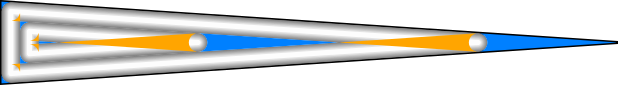
\includegraphics[width=\figwidth]{sources-intro-TEST-naive-accuracy.png}
\end{subfigure}
\begin{subfigure}{\figwidth}\centering
\parbox[b]{\figwidthTwo}{\subcaption{}\label{intro_wedge_centered}}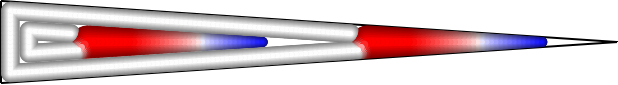
\includegraphics[width=\figwidth]{sources-intro-TEST-Center-widths.png}
\end{subfigure}
\begin{subfigure}{\figwidth}\centering
\parbox[b]{\figwidthTwo}{\subcaption{}\label{intro_wedge_distributed}}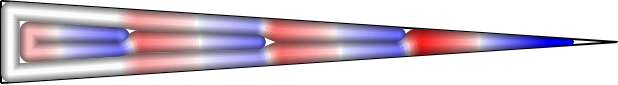
\includegraphics[width=\figwidth]{sources-intro-TEST-Distributed-widths.png}
\end{subfigure}
\caption{
Illustration of different toolpath\revise{}{s} for a \revise{wedge }{}shape \revise{}{showcasing a range of shape radii }\revise{}{(black)}.
\revise{}{These results can be read as a graph with feature size on the horizontal axis and its corresponding beading along the vertical axis.}
\subref{intro_wedge_uniform} Toolpath using uniform offsetting results in large overfill (orange) and underfill (azure).
\subref{intro_wedge_centered} Toolpath with adaptive width~\cite{Jin2017JMS} where beads that are wider or narrower than the nozzle size are indicatd in red and blue, respectively.
\subref{intro_wedge_distributed} Our approach minimizes over- and underfill with \revise{beads close to the nozzle size}{less extreme widths}.
}
\label{intro_wedge}
\end{figure}

\paper{4. Beading schemes, end of section}{
\paragraph{Widening \revise{}{meta-scheme}}
Complementary to any of these schemes we can enforce a minimum feature size \revise{at no extra cost}{and minimum bead width} in our framework.
Regions where the model is narrower than \revise{the nozzle size}{some $r_\text{min}$} can be printed with a bead width \revise{}{$w_\text{min}$} larger than the model thickness.
See \cref{min_feature_size} and~\subref{widening}.
We can simply override
\begin{align*}
q'(d) &= 
\begin{cases}
0 & \text{ if } 0 \leq d < 2 r_\text{min} \\
1 & \text{ if }  2 r_\text{min} \leq d < w^*  \\
q(d) & \text{ otherwise}
\end{cases}
\\
W'(n,r)_0 &=
\begin{cases}
\max \left( w_\text{min}  ,  2 r \right) & \text{ if } 2 r < w^* \\
W(n,r)_0 & \text{ otherwise}
\end{cases}
\end{align*}



\revise{}{
\paragraph{Shell meta-scheme}
The industry standard of FDM is to generate only a limited contour-parallel perimeters and to fill the remainder using a direction-parallel strategy.
We therefore provide a meta-scheme to generate adaptive bead width toolpaths only in narrow regions and generate the limited number of perimeters $M$ using the preferred width in regions which are wide enough.
We also take care not to leave gaps which are too small to be filled using the direction-parallel strategy:
}

\revise{}{
\begin{align*}
q'(d) &= \min(M, q(d))
\\
W'(n,r)_i &= 
\begin{cases}
W(n, M w^*)_i & \text{ if } 2 r > q^{-1}(M) \\
W(n,r)_i & \text{ otherwise}
\end{cases}
\end{align*}
}

\revise{}{
These meta-schemes introduce non-linearities in the quantization function.
Because the beading is only evaluated at nodes in the skeleton, we need to make sure that there are nodes at the locations along the skeleton where the non-linearities happen.
We therefore insert extra nodes along with their ribs at locations $v$ with a radial distance $R(v) = r_\text{min}$ for widening and at $R(v) \in \left\{ M w^*, q^{-1}(M), q^{-1}(M) + \nicefrac12 w^* \right\} $ for the transition from narrow shell to unconstrained shell.
Combining all meta-schemes functionality we can generate results such as depicted in \cref{shell}.
}
\begin{figure}
\centering
\setlength{\figwidth}{.35\mycolumnwidth}
\setlength{\figwidthTwo}{.6\mycolumnwidth}
\begin{minipage}[b]{\figwidthTwo} \centering
\begin{subfigure}[b]{\figwidthTwo}\centering
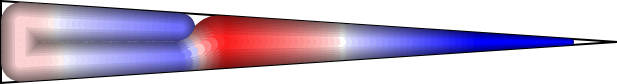
\includegraphics[width=\figwidthTwo]{sources-validation-wedge-TEST-Distributed-feature-size.png}
\caption{Widening meta-scheme using $w_\text{min} = 2 r_\text{min} = 0.1$
\\ on top of the Distributed scheme}
\label{min_feature_size}
\end{subfigure}
\begin{subfigure}[b]{\figwidthTwo}\centering
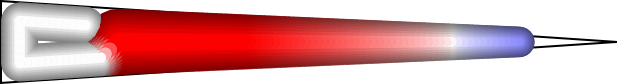
\includegraphics[width=\figwidthTwo]{sources-validation-wedge-TEST-Center-widening.png}
\caption{Widening meta-scheme using $w_\text{min} = 0.5$, $2 r_\text{min} = 0.2$ 
\\ on top of the Center scheme}
\label{widening}
\end{subfigure}
\end{minipage}
\begin{subfigure}[b]{\figwidth}\centering
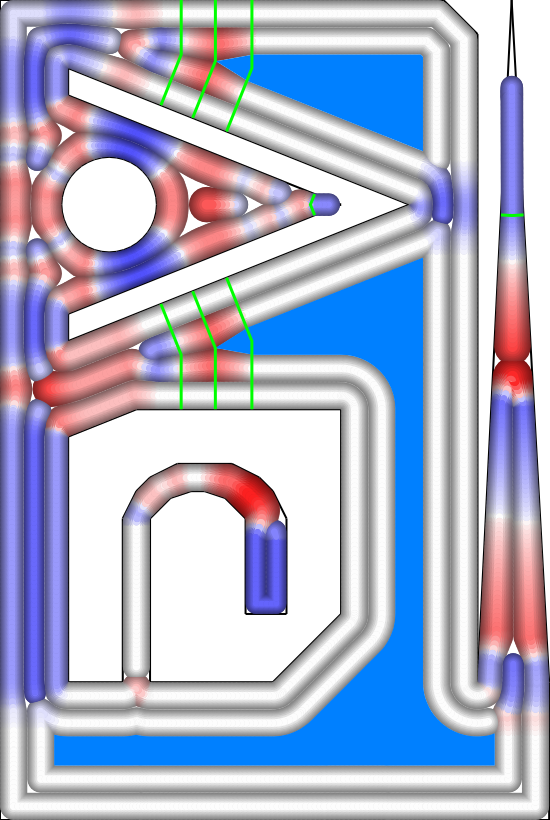
\includegraphics[width=\figwidth]{sources-validation-gMat_example_all_combined.png}
\caption{Shell and widening}
\label{shell}
\end{subfigure}
\caption{
Toolpaths using the widening and shell meta-schemes.
\subref{min_feature_size} and~\subref{widening} show widening.
\subref{shell}
show toolpaths generated with the inward distributed strategy ($N=1.5$) in conjunction with the shell meta-scheme ($M=4$) and the same widening as in~\subref{widening}.
% -p test_geometry/gMAT_example.svg -b 4 -s i -n 1.5 -a --mins 0.2 --minw .5
Widening and shell require extra edges (green) at key locations in the skeleton.
The azure area is to be filled using some direction-parallel toolpaths.
}
\label{widening_shell}
\end{figure}
}
\paper{5.2 Computational results}
{
Toolpaths of these 300 outline shapes are generated using the uniform technique as implemented by Clipper~\cite{johnson2014clipper} -- a state-of-the-art polygon offset library,
and by our framework using four beading schemes, i.e. the constant bead count scheme with a bead count of $C=4$, the centered, the evenly distributed, and the inward distributed beading scheme using \revise{$N=3$}{$N=2$}, all with a preferred bead width\revise{s}{} of \revise{$w^* = \SI{0.4}{\milli\meter}$}{$w^* = \SI{0.5}{\milli\meter}$ and using the widening meta-scheme to enforce a minimum printed feature size of $w_\text{min}=2r_\text{min}=\SI{0.3}{\milli\meter}$}.
}




\subQue{
If there is no sharp corners exist, then the existing approaches such as Jin et al (2017) do not have to use bead widths of large variations. 
}
\Ans{
The wedge shape of Fig. 1 was chosen because it contains a wide range of feature sizes and is therefore representative for a wide range of models.
Nearly every model induces the full range of $[0.5w^*,1.8w^*]$ using the centered approach by Jin et. al. 2017 JMS,
because nearly all models have feature sizes which span any range $[iw^*,(i+1)w^*]$ for $i\in\mathcal{N}$.
See Fig. 17 in the paper of Jin et al for an example shape.
Only shapes without central regions (a circle) or shapes with central regions with an exact multiple of $w^*$ everywhere (a rectangle) don't require any variation in bead width, but that holds for any of the beading schemes.

Figure~\ref{no_corners} shows an example of a shape without sharp corners, and which also requires a large bead width variation when using the constant bead count approach by Ding et al.
}
\begin{figure} \centering
\setlength{\figwidth}{.45\mycolumnwidth}
\begin{subfigure}[b]{\figwidth} \centering
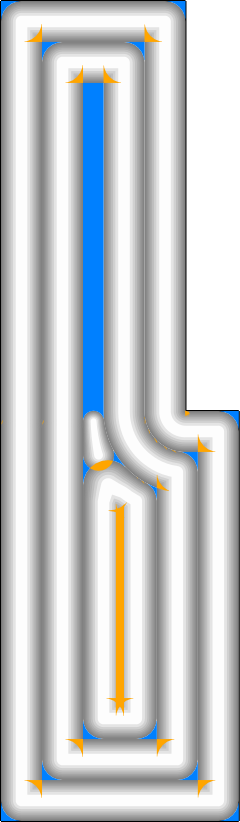
\includegraphics[rotate=-90,width=\linewidth]{response_rects_Center_accuracy.png}
\caption{Problematic for center, i.e. Jin et al 2017 JMS, exhibiting $4.5w^*$ and $5.8w^*$}
\end{subfigure}
\begin{subfigure}[b]{\figwidth} \centering
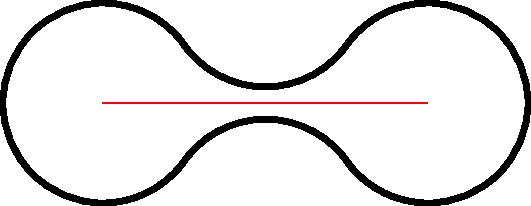
\includegraphics[width=\linewidth]{response_no_corners}
\caption{Problematic for constant, i.e. Ding et al}
\end{subfigure}
\caption{Example shapes without sharp corners.}
\label{no_corners}
\end{figure}





\Que{
How do the authors conduct path planning? Could the authors add a simple 2D geometry with multiple holes to explain the path planning process? As the proposed approach adds more disconnected toolpaths to minimize underfill areas, an improper path planning would significantly increase the fabrication time. 
}
\Ans{
We now included a description of the path order algorithm, which is naive and greedy.
Although an optimal path order algorithm might influence the travel time, such an algorithm is slow and not generally used in the industry.
The software package Cura currently employs a similarly greedy algorithm.
Travel times are approximately \SI{2}{\percent} of the total print time in our current setup, so the effect of improper path planning is negligible compared to the differences in extrusion time.

We now include statistics on extrusion time, travel time and path counts.
These new statistics are now also reflected upon in the comparison of the beading schemes.

Because the extrusion time depends on the actual printing setup we have moved the section on print results to before the statistics section.
}
\commits{
d375878a8a6d01c53436aeb9c473dbedd8f3edcf % path order algorithm
e2c940f2362556ae8d017cff63c81b4bbcb77286 % print time, path count statistics
7f567012b409445fc120968e995f861cab56e776 % new beading schemes comparison
bf403fe797193e40b004c2cae806935f699271e5 % move print results to before statistics 
b106dd1e0067114756bf96a7dc10458202380f2e % new print time pdf graph
}
\paper{5.1.2 Print results}{\revise{}{The printing order is determined greedily by choosing the closest point of a polygonal extrusion path, or the closest of either end point in case of an open polyline extrusion path.}} 
\paper{5.2.3 Print time}
{
\revisepar{
\subsubsection{Smoothness of toolpaths}
In order to maintain a high printing speed, it is desirable that toolpaths have fewer and less sharp corners. 
We therefore measured the angle between consecutive extrusion segments generated by each scheme
and report on the occurrence of each angle in \cref{smoothness}.
All schemes show a higher number of corners for smaller angles with a peak towards \SI{180}{\degree} (straight).
We observe that compared to the uniform method our framework produces less acute angles which, but more obtuse angles.
The inward distributed scheme produces an order of magnitude less corners around \SI{150}{\degree}, compared to evenly distributed. 
We also investigated the effect of the transition regions on the smoothness of the toolpaths. 
\cref{smoothnessNoTransition} shows that introducing the transitions greatly reduces the number of corners around \SI{90}{\degree}. 
}{
\subsubsection{Print time}
The total time it takes to print a part is influenced not only by our back pressure compensation scheme, but also by the geometry of the toolpaths.
In order to separate these effects we report on the total print time when using back pressure compensation and when using a constant (maximum) movement speed in \cref{printtime}.
We estimate print times using a simulation of the Marlin firmware using the default movement settings of the setup described in \cref{print_results_section}.
While the idealized print time is predominantly determined by the total toolpath length, the print time using back pressure compensation is predominantly determined by the occurrence of wide beads, because they have a reduced the flow in \si{\milli\meter\cubed\per\second}.
Because of acceleration constraints imposed by the hardware the maximum movement speed is not reached near sharp corners.
We therefore also report on the angles of the bends in the toolpaths in \cref{smoothness}.
Furthermore, the print time is negatively affected by discontinuities in the extrusion process.
Between extrusions the printer needs to stop extrusion, travel to the next extrusion path and restart the extrusion process, which all take time.
For closed polygonal toolpaths we can start anywhere within the path, so we can optimize the starting location so as to minimize the travel time.
We therefore report both on the open and closed path count in \cref{pathcounts}.
}
}
\paper{5.3 Comparison of beading schemes}
{
We can see from \cref{TEST_naive_accuracy}(top) and~\ref{over_underfill} that the uniform technique causes a lot of overfills and underfills: on average \revise{approximately}{} \revise{\SI{1}{\percent}}{\SI{1.6}{\percent}} of the total target area is covered by underfill and likewise for overfill.
To our knowledge, the uniform beading scheme, as well as the outer beading scheme, is of little use to FDM printers.

The constant bead count scheme effectively deals with underfills, but generates orders of magnitude more overfills compared to the other schemes. 
Also, the scheme comes at the cost of greatly varying bead widths and an average bead width that is not close to the preferred bead width.
Note that most overfill areas occur near regions of alternating bead width. 
\revise{}{While the scheme results in short toolpaths, as indicated by the idealized print time, it also results in a wide range of bead widths, which cause the back pressure compensation print time to be very large.
See \cref{statisticsfig}.}
For an input outline shape which contains both very small and very large features, the constant bead count scheme produces bead widths which can fall outside of the range of manufacturable bead widths.
Moreover the centrality marking is not robust against small perturbations in the outline; adding a small chamfer in a corner causes the unmarked ST to be very small at that location, which results in tiny bead widths.
\revise{}{See top right of \cref{TEST_Constant_accuracy}.}

In \cref{TEST_Center_accuracy} we can see that
the centered beading scheme effectively deals with \revise{both }{}overfill \revise{and underfill }{}and produces desired bead widths in all locations, except for the extrusion paths in the center, where the bead widths \revise{are within a factor 2 off from the desired bead width.}{range between $0.5 w^*$ and $1.8w^*$, i.e. the variation is within a factor of $3.6$.}
\revise{}{However, it does produce some narrow underfill regions.}
\revise{
According to \cref{over_underfill} the overfill and underfill for the centered, the evenly distributed and the inward distributed scheme are all approximately \SI{0.2}{\percent}, which is a considerable improvement over the uniform technique.
}{
Compared to the uniform technique the centered technique increases the (open) path count, but considerably reduces over- and underfill and decimates the number of toolpath angles below \SI{45}{\degree}.
See \cref{statisticsfig}.
}

However, according to \cref{widthHistogram} the centered scheme exhibits a wider range of bead widths than the distributed schemes:
the standard deviation of the bead widths in the centered scheme is approximately \SI{39}{\micro\meter}, while that of the distributed schemes is approximately \SI{14}{\micro\meter}.%_
\revise{}{\footnote{\revise{}{Although the standard deviation $\sigma$ of the inward distributed scheme is slightly higher, the mean absolute deviation is lower than that of the evenly distributed scheme (i.e. \SI{9}{\micro\meter} versus \SI{11}{\micro\meter}), because its distribution is more peaked.}}}
\revise{}{Moreover, because the quantization operator rounds to the nearest number of beads, in the worst case where we switch from a single to two beads the widths switch from $0.75w^*$ to $1.5w^*$, i.e. the variation is within a factor $2$, which is considerably lower the than factor of $3.6$ in the centered scheme.}
We therefore conclude that the distributed schemes \revise{result in bead widths closer to the preferred widths}{exhibit a lower bead width variation and lower (open) path count} compared to the centered scheme.
%This is desirable for the manufacturability of the beads and can therefore have a positive effect on the mechanical properties and surface quality of the 3D prints. 

\revise{It is hard to visually identify the difference between the evenly and the inward distributed scheme in \cref{visualized_accuracy}, because that particular example shape does not have wide features.}
{\Cref{distributed_comparison,TEST_Distributed_accuracy,TEST_InwardDistributed_accuracy} show that in the inward distributed scheme the outer toolpaths have the preferred width more often than in the evenly distributed scheme, which means that the outline acuracy of the inward distributed beading is less affected by inaccuracies in the adaptive width control system.}
%{\Cref{TEST_InwardDistributed_accuracy} shows that in the inward distributed scheme the outer beads are more often equal to the preferred width compared to the evenly distributed scheme in \cref{TEST_Distributed_accuracy}, but that effect is more pronounced for wider geometry such as in \cref{distributed_comparison}.}
%While the difference between the evenly and inward distributed scheme in \cref{visualized_accuracy} results only in the outer bead being the preferred width in some locations, the effect of the inward distributed scheme is more pronounced in larger geometry, as can be seen in \cref{distributed_comparison}.}
\revise{However, \cref{distributed_comparison} and  \cref{widthIndexedHistogram} confirm that the outer toolpaths have the preferred bead width more often.}{} % _
Furthermore, \revise{from \cref{smoothness} }{}we find that compared to evenly distributed, the inward distributed scheme produces \revise{smoother toolpaths overall}{less corners with angles above \SI{130}{\degree} and less overfill, because the area of influence that bead count transitions have is limited in the inward distributed scheme}.
Thus the inward distributed scheme prevents over- and underfill, generates smooth toolpaths with more homogeneous width and affects smaller more centered parts of the print than the other schemes\revise{}{, while incurring little to no extra print time}. 
}









\begin{figure*}
\centering
\setlength{\figwidth}{0.19\textwidth}
\setlength{\figheight}{0.283\textwidth}
\begin{subfigure}{\figwidth}\centering
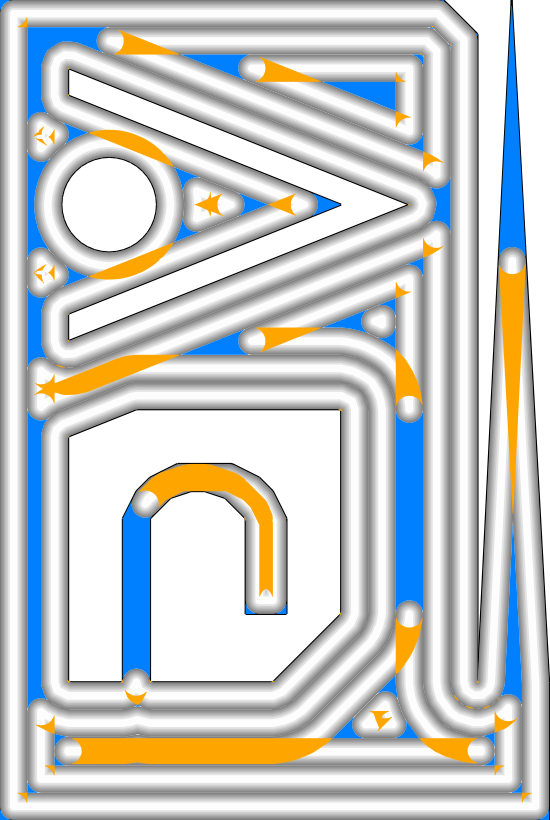
\includegraphics[height=\figheight]{sources-validation-gMAT-example-TEST-naive-accuracy.png}
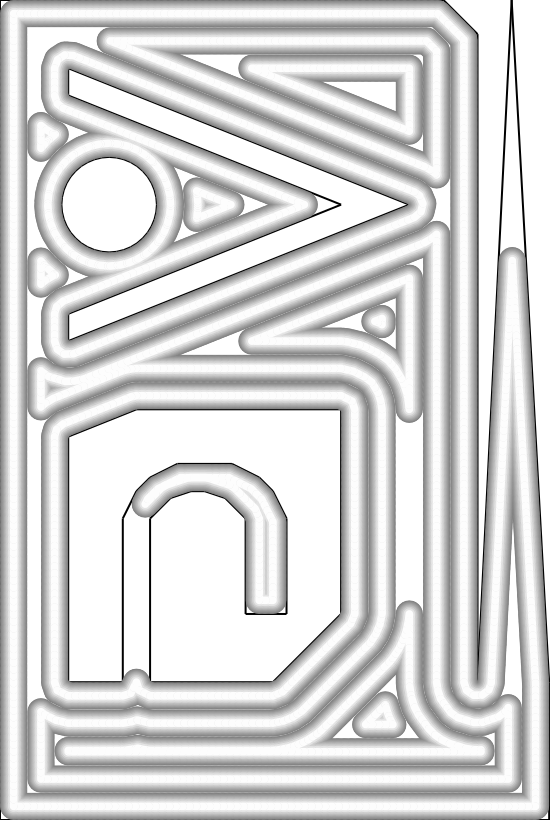
\includegraphics[height=\figheight]{sources-validation-gMAT-example-TEST-naive-widths.png}
\caption{Uniform}\label{TEST_naive_accuracy}
\end{subfigure}
%\begin{subfigure}{\figwidth}\centering
%\includegraphics[height=\figheight]{sources-validation-gMAT-example-TEST-SingleBead-accuracy.png}
%\includegraphics[height=\figheight]{sources-validation-gMAT-example-TEST-SingleBead-widths.png}
%\caption{Single}\label{TEST_SingleBead_accuracy}
%\end{subfigure}
\begin{subfigure}{\figwidth}\centering
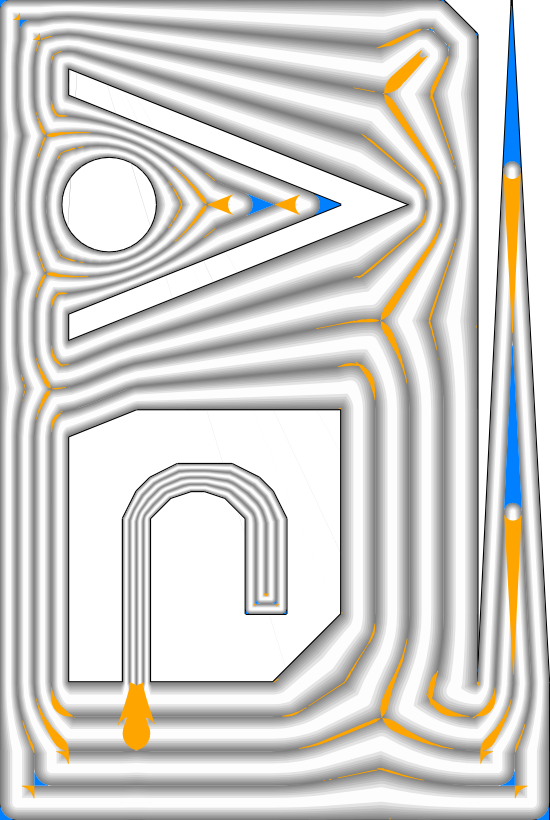
\includegraphics[height=\figheight]{sources-validation-gMAT-example-TEST-Constant-accuracy.png}
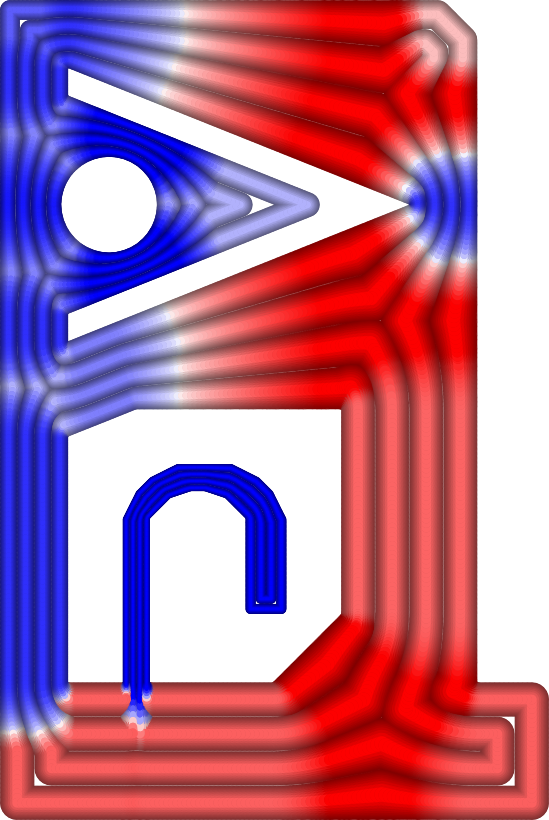
\includegraphics[height=\figheight]{sources-validation-gMAT-example-TEST-Constant-widths.png}
\caption{Constant}\label{TEST_Constant_accuracy}
\end{subfigure}
\begin{subfigure}{\figwidth}\centering
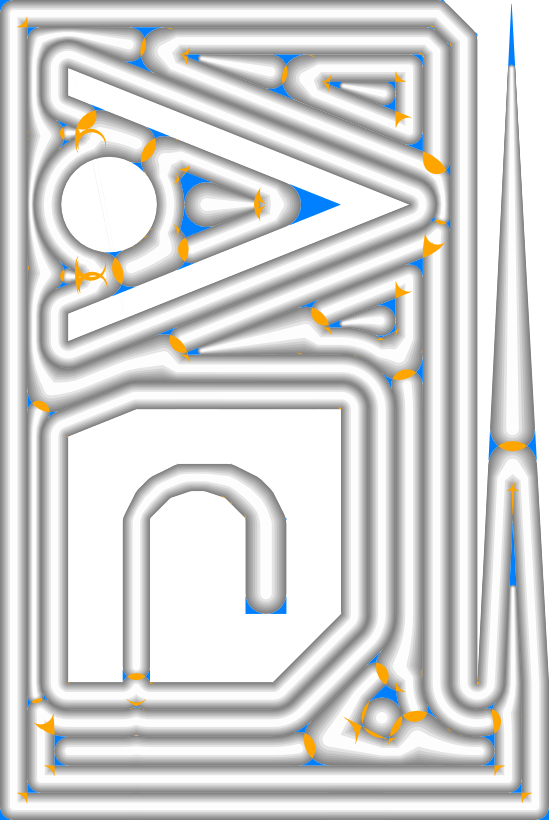
\includegraphics[height=\figheight]{sources-validation-gMAT-example-TEST-Center-accuracy.png}
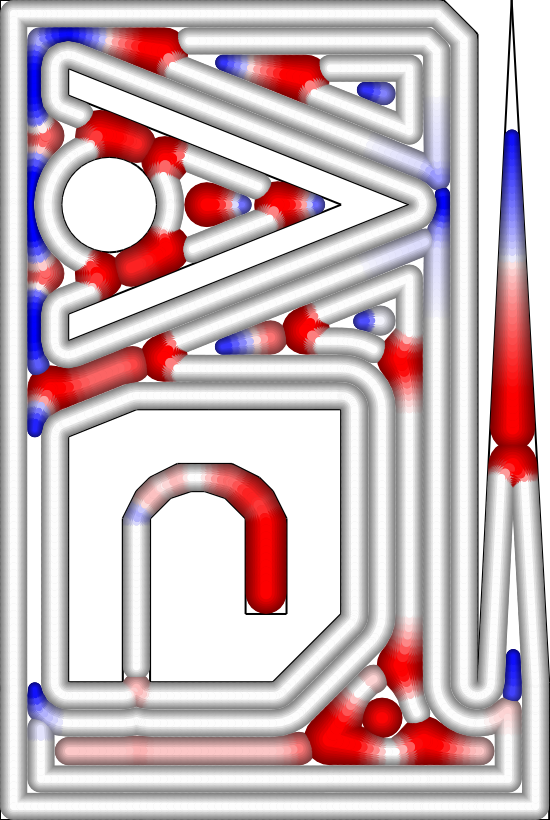
\includegraphics[height=\figheight]{sources-validation-gMAT-example-TEST-Center-widths.png}
\caption{Centered}\label{TEST_Center_accuracy}
\end{subfigure}
\begin{subfigure}{\figwidth}\centering
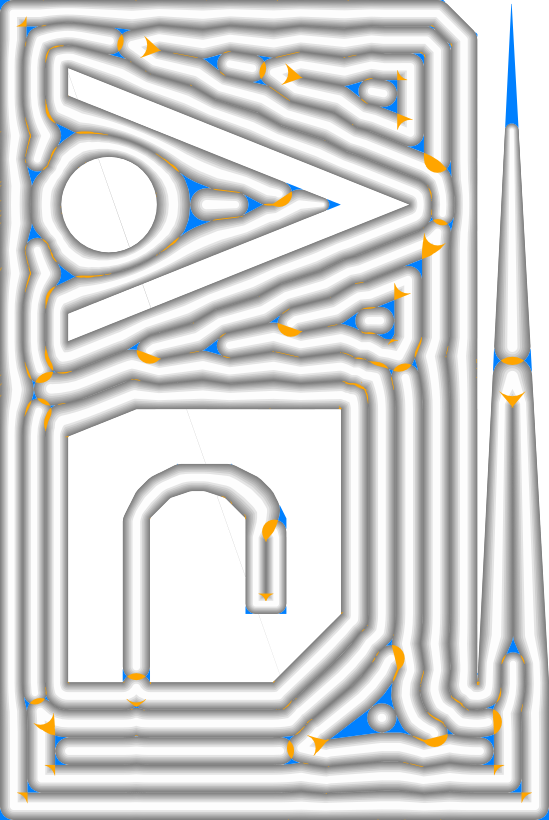
\includegraphics[height=\figheight]{sources-validation-gMAT-example-TEST-Distributed-accuracy.png}
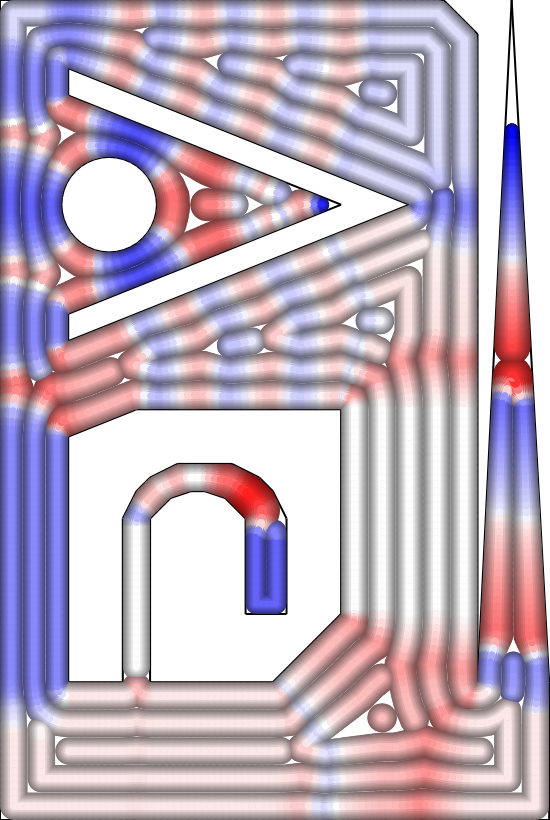
\includegraphics[height=\figheight]{sources-validation-gMAT-example-TEST-Distributed-widths.png}
\caption{Distributed}\label{TEST_Distributed_accuracy}
\end{subfigure}
\begin{subfigure}{\figwidth}\centering
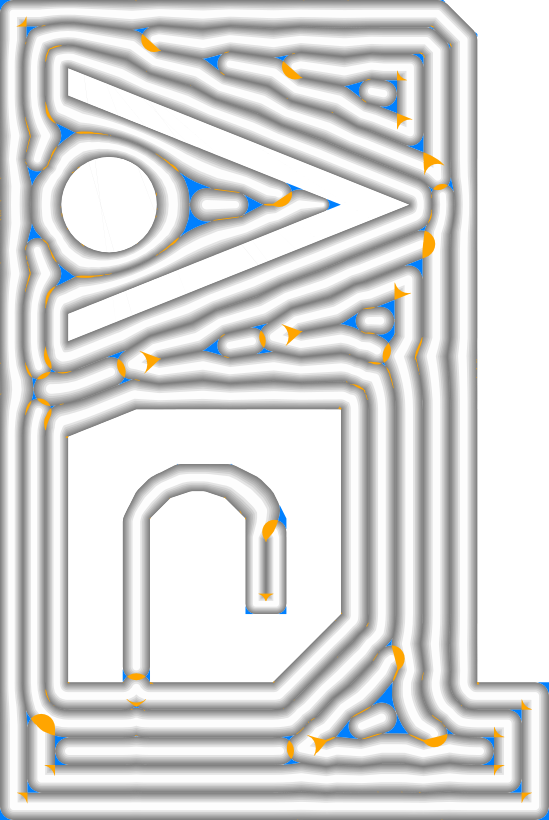
\includegraphics[height=\figheight]{sources-validation-gMAT-example-TEST-InwardDistributed-accuracy.png}
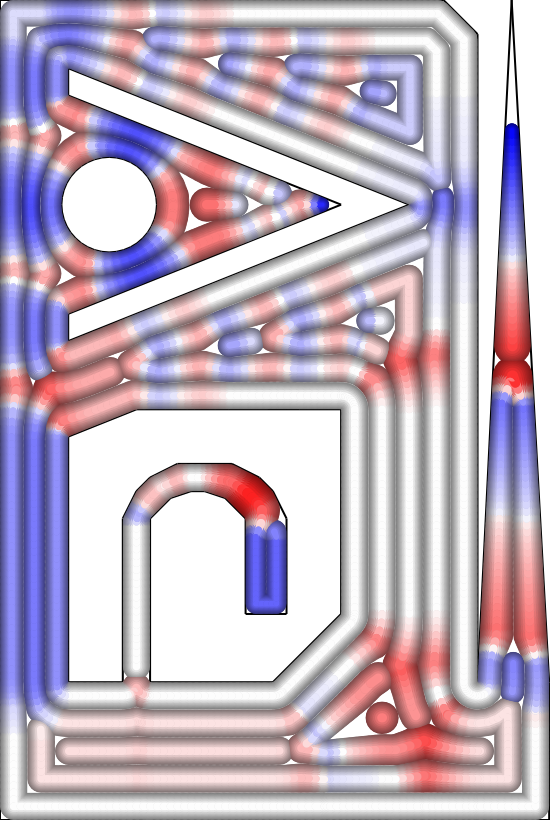
\includegraphics[height=\figheight]{sources-validation-gMAT-example-TEST-InwardDistributed-widths.png}
\caption{Inward \revise{}{($N=2$)}}\label{TEST_InwardDistributed_accuracy}
\end{subfigure}
\begin{subfigure}{.04\mycolumnwidth}\centering
\vspace{4.7cm}
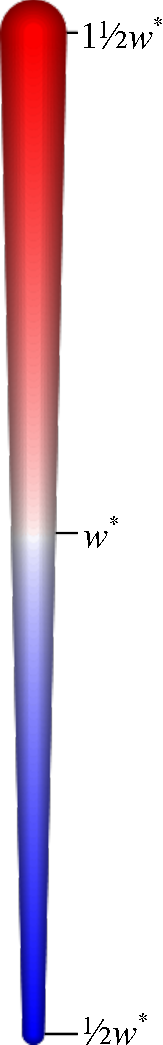
\includegraphics[height=\figheight]{sources-validation-gMAT-example-widths-legend.pdf}
\end{subfigure}
\caption{
Visualization of the overfills and underfills (top) and the widths (bottom) for various beading schemes.
Extrusion beads in gray tones,
overfill in orange,
underfill in azure,
narrow beads in blue
and wide beads in red.
\revise{New shape contains pointy wedge to see impact on minimal feature size}{In order to distinguish clearly from the Distributed scheme the Inward is limited to $N=2$.}
}
\label{visualized_accuracy}
\end{figure*}




\begin{figure*}
\centering
\setlength{\figheight}{0.25\textwidth}
\setlength{\figwidth}{0.32\textwidth}
\begin{subfigure}{\figwidth}\centering
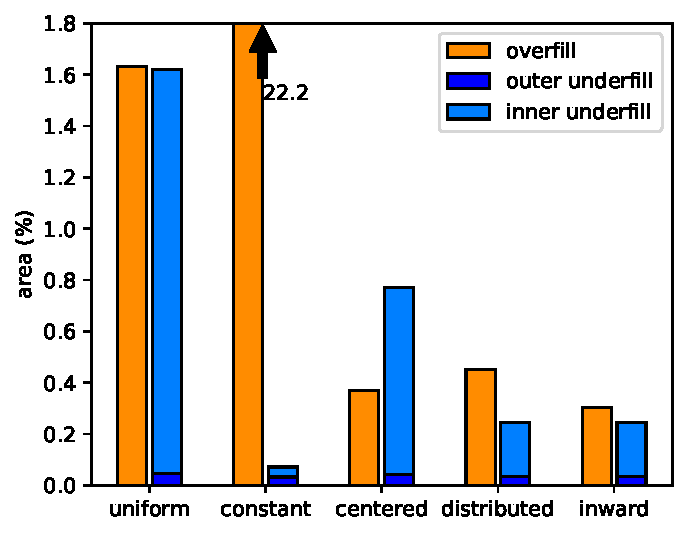
\includegraphics[height=\figheight]{sources-validation-over-underfill.pdf}
%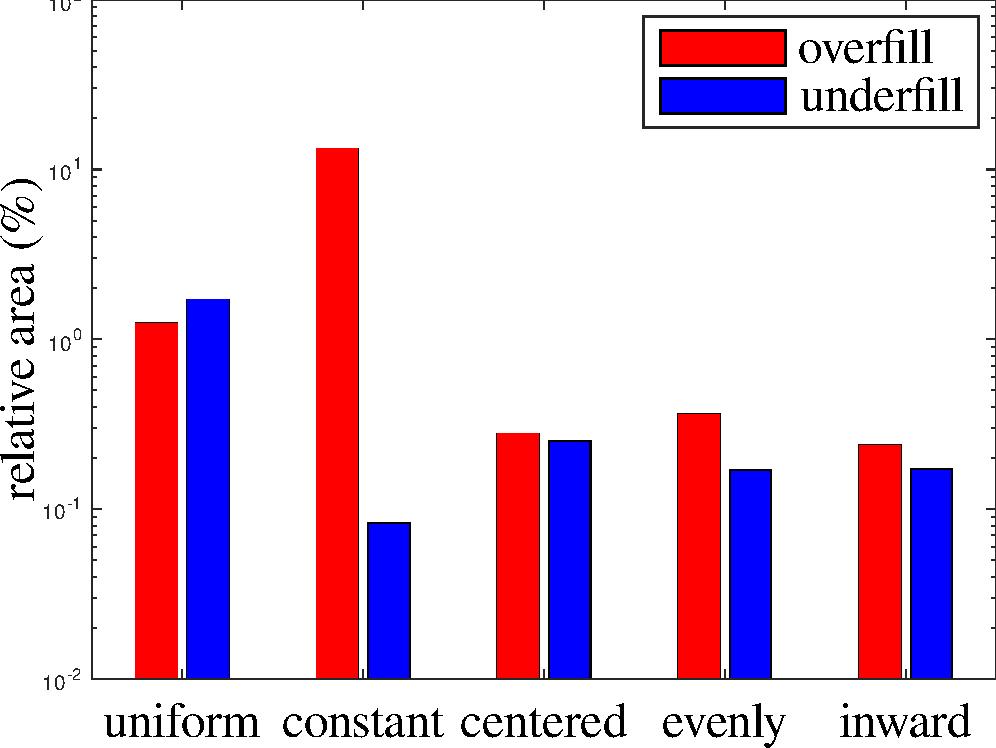
\includegraphics[width=\figwidth]{sources-validation-overunderfill.pdf}
\caption{\revise{}{Over- and underfill}}
\label{over_underfill}
\end{subfigure}
\begin{subfigure}{\figwidth}\centering
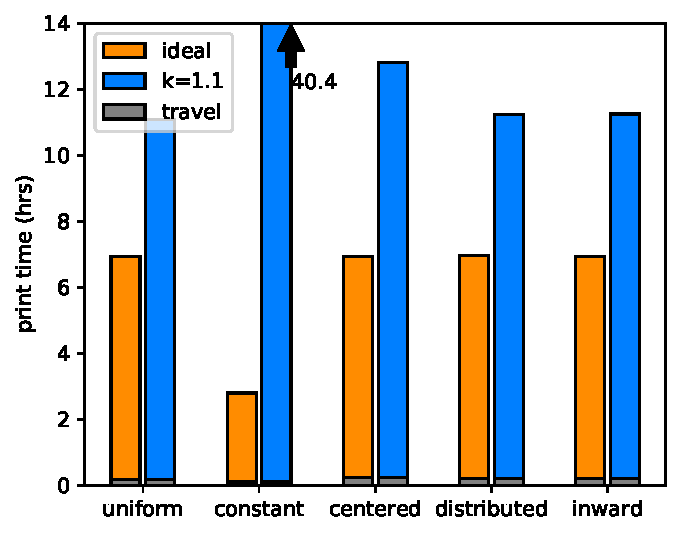
\includegraphics[height=\figheight]{sources-validation-print-time.pdf}
%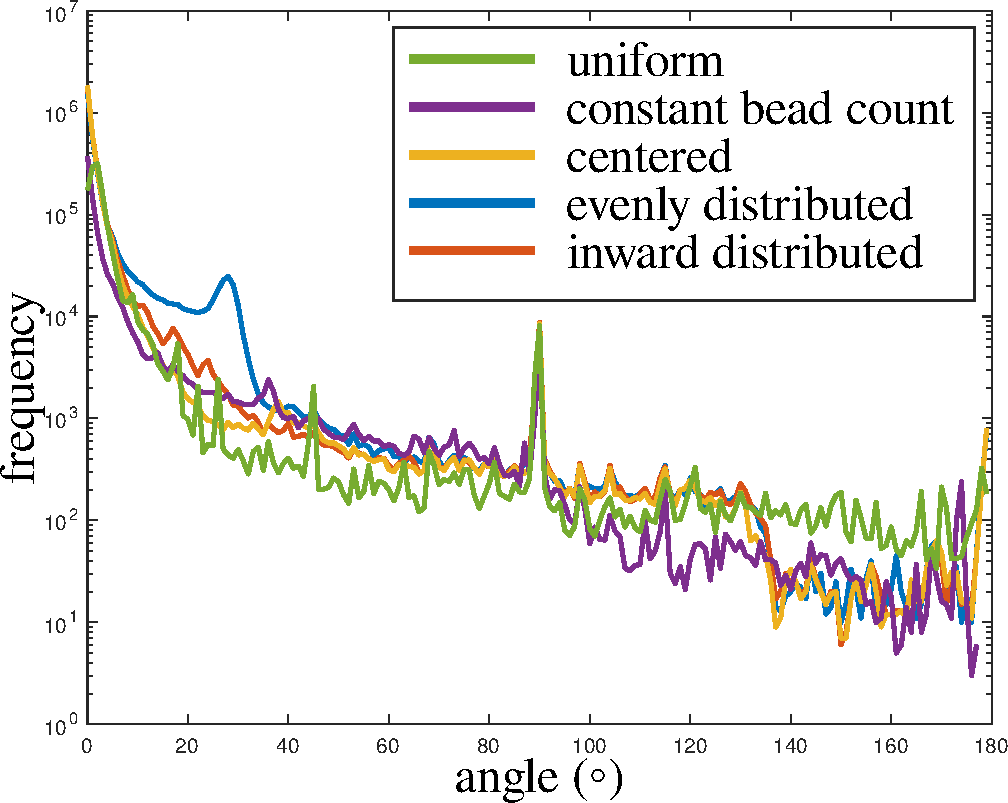
\includegraphics[width=\figwidth]{sources-validation-smoothness.pdf}
\caption{\revise{}{Print time}}
\label{printtime}
\end{subfigure}
\begin{subfigure}{\figwidth}\centering
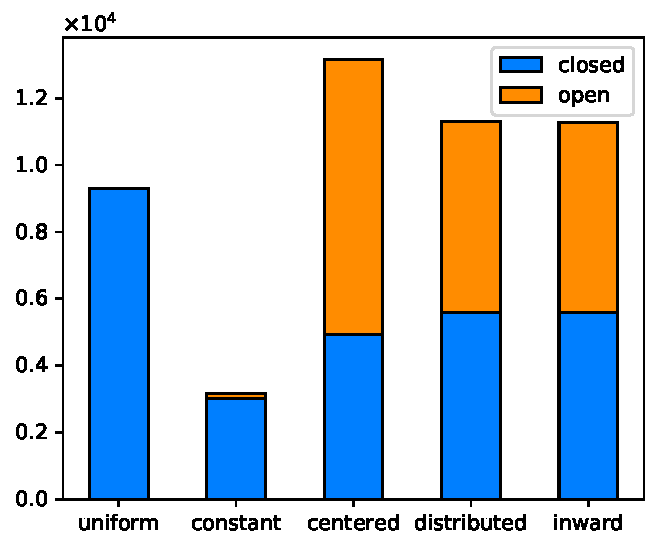
\includegraphics[height=\figheight]{sources-validation-path-counts.pdf}
%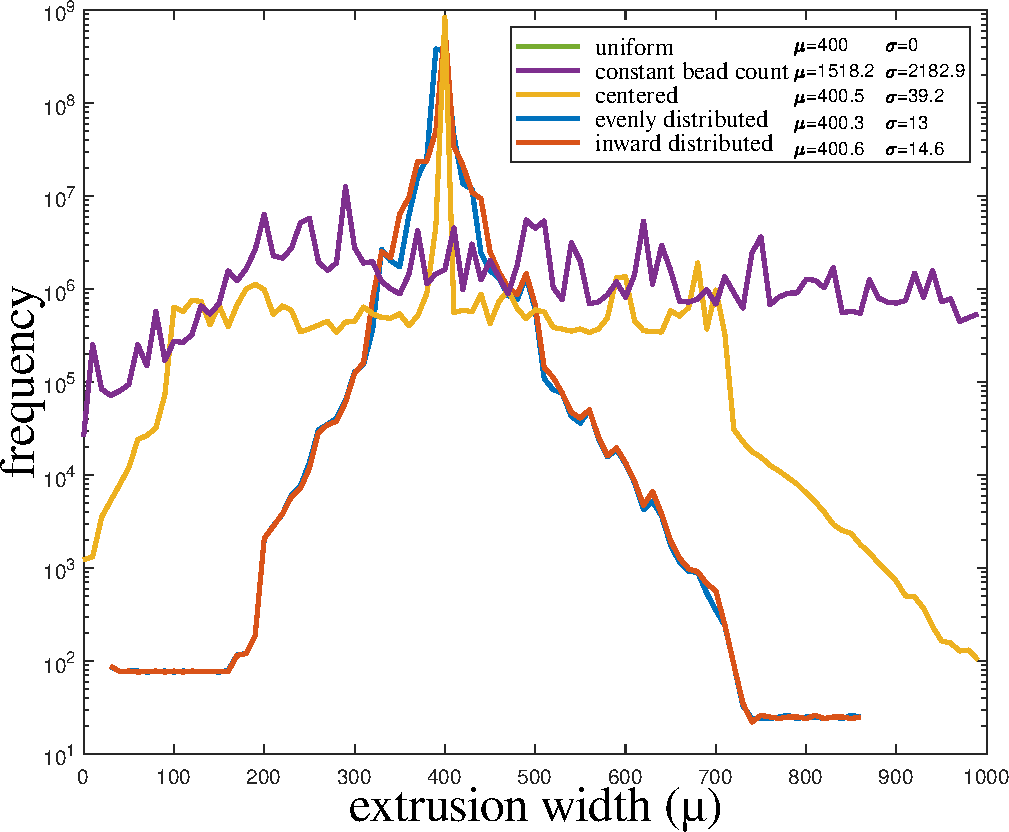
\includegraphics[width=\figwidth]{sources-validation-widthHistogram.pdf}
\caption{\revise{}{Path counts}}
\label{pathcounts}
\end{subfigure}

\begin{subfigure}{\figwidth}\centering
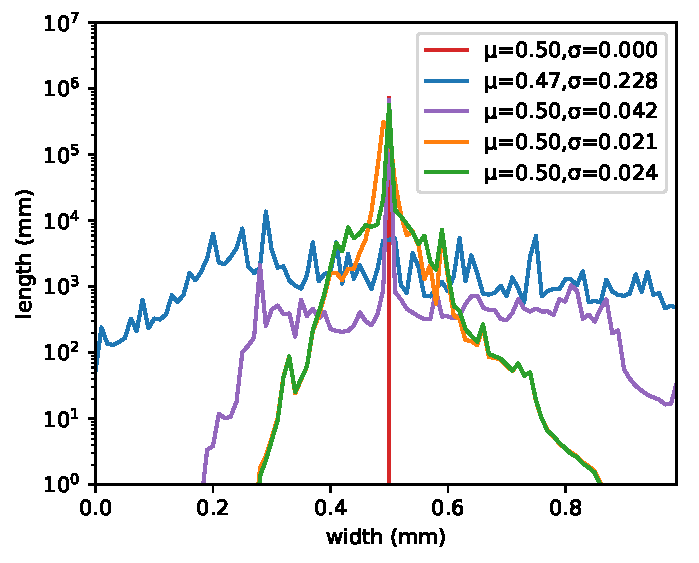
\includegraphics[height=\figheight]{sources-validation-widths.pdf}
%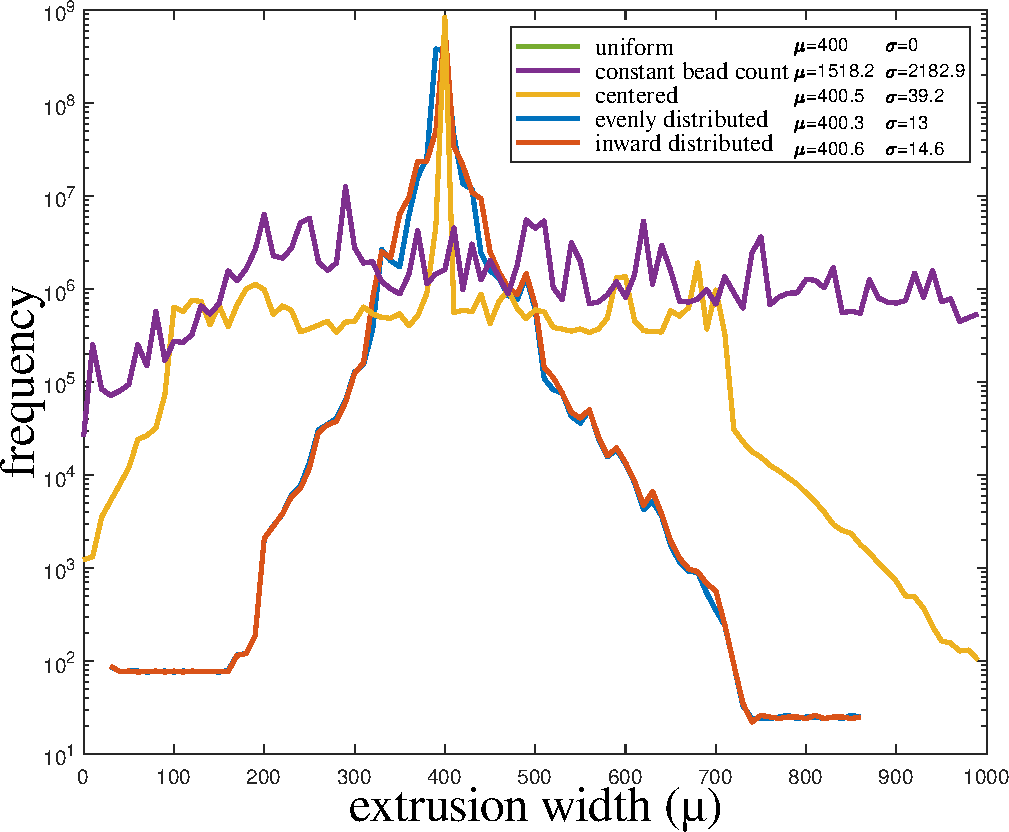
\includegraphics[width=\figwidth]{sources-validation-widthHistogram.pdf}
\caption{\revise{}{Extrusion widths}}
\label{widthHistogram}
\end{subfigure}
\begin{subfigure}{\figwidth}\centering
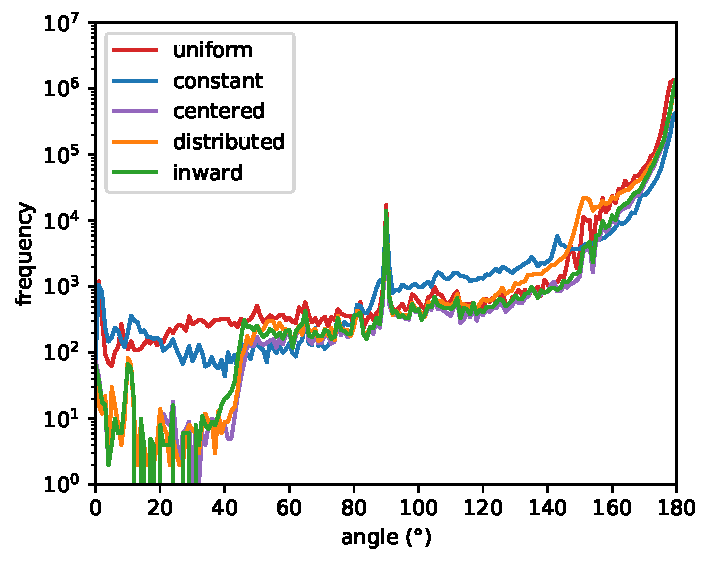
\includegraphics[height=\figheight]{sources-validation-angles.pdf}
%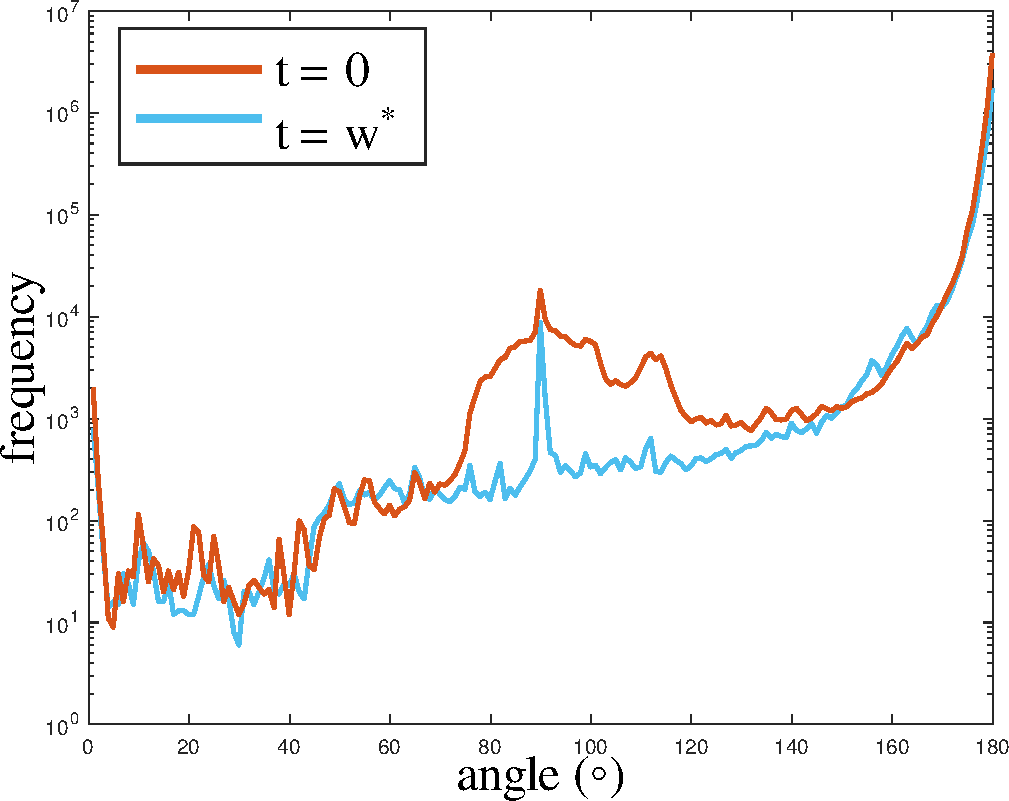
\includegraphics[width=\figwidth]{sources-validation-smoothnessNoTransition.pdf}
\caption{\revise{}{Site angles}}
\label{smoothness}
\end{subfigure}
\begin{subfigure}{\figwidth}\centering
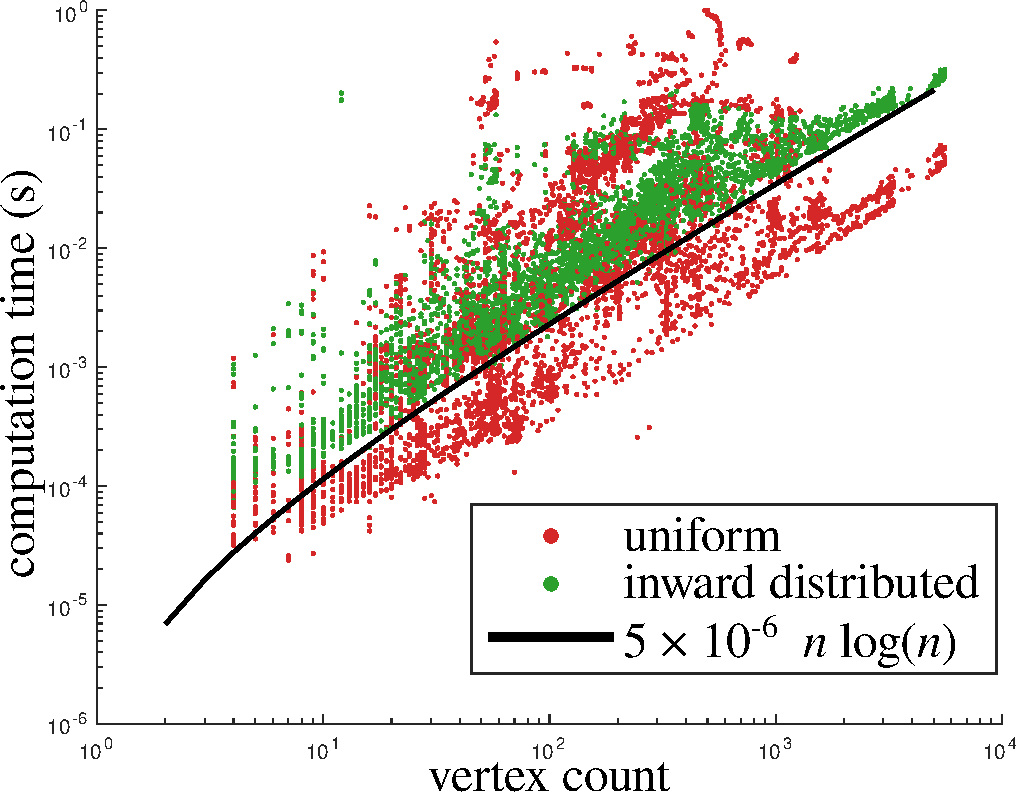
\includegraphics[height=\figheight]{sources-validation-computime2.pdf}
%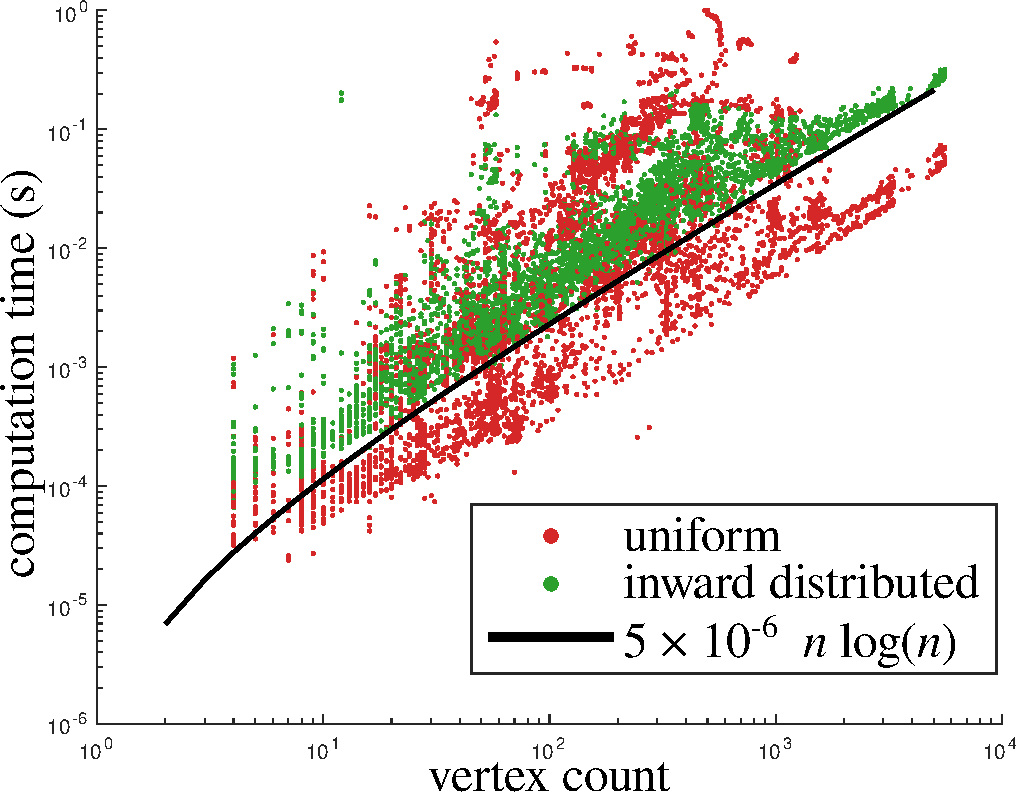
\includegraphics[width=\figwidth]{sources-validation-computime2.pdf}
\caption{Computation time}
\label{computime}
\end{subfigure}


\caption{
Statistical analysis of the toolpaths from applying the uniform width technique and various beading schemes using our framework to a data set of 300 slices.
Note the use of a logarithmic scale \revise{}{in the bottom graphs }on the Y-axes and \revise{on some of}{for \subref{computime} on} the X-axes as well.
}
\label{statisticsfig}
\end{figure*}











\Que{
While the proposed approach can use adaptive bead width to minimize underfill and overfill areas, the generated toolpaths are disconnected compared to the traditional approaches. From my experience, a small overfill area does not have to lead to serious defects. But the disconnected filaments definitely have worse mechanical performances compared to the continuous ones. 
}
\Ans{
That is a difficult question.
It might very well be true that discontinuous extrusion lines form a bigger problem than some over- or underfill areas - at least certainly for flexible filaments on a Bowden printer.
However, it is quite hard to find a mathematical approach to balance discontinuity with the size of over-/underfill areas.

%It should be noted that even small underfill areas can be unfillable using an overextrusion approach.
%For example the microgaps at 3-way intersections.
%The viscocity of molten filament is too high to reach into those small crevices.
}
\todo{
count number of extrusion toolpaths?

That might be true, but the microgaps near 3-way intersections are not fillable using overfilling; the plastic cannot creap into those cravices.
}
\commits{
f2132c1c0cbce6daa29f64890be5f9e20c79c630 % future work notice
}




\Que{
Why the authors state the inward distributed beading scheme as new? Jin et al (2017) has proposed the strategy to add a toolpath with varying width along the center edges of the skeleton, and with unchanging width outside.
}\label{difference_to_jin}
\Ans{
The difference between the inward distributed beading scheme and the method by Jin et al 2017 JMS is already shown in Fig 1.b and c. 
It is also shown in Fig. 18 c and e.
In order to clearly address the difference early on we mention the difference in the description of Jin in the introduction.
}
\commits{b7c4d299a76e9fab6c233d572f3248c1350a2e8c}
\paper{Intro}{
\revise{
Therefore, a narrower range of widths is desirable.
}
{We therefore reduce the bead width range by distributing the workload from the centermost bead over neighboring beads.}
}





\Que{
In Fig.1, how to justify the proposed approach as different geometries are used? I believe if the authors use the same geometries as in Fig 1. (a) and (b), there would be also underfill areas using the proposed approach. 
}\label{fig1geometry}
\Ans{
There are two ways in which we can interpret this question, leading to two responses.
The question can be interpreted as saying that Fig a has a different geometry than b or c.
There is now a black outline to show that the shapes in Fig 1a, b and c are actually the same geometry, and the output is less confusing because we now use the same minimum feature size for b and c.

The question can also be interpreted as saying that one might use a different shape than the geometry in Fig 1.
We decided on this wedge shape because it shows how the techniques deal with a wide range of feature sizes;
the wedge shape can be read as a graph where we can read out the resulting beading for any local feature size.
}
\commits{45853e8b30d93f60e9465cbb649e347f9cfc23b1 53224c04ceff6c1b18a9eea6de8e7e33957b7797}
\paper{Intro}{
[See caption of \cref{intro_wedge}.]
}



\Que{
Please double check the following sentences. ”Third, the extruded path should ...”(at the second paragraph of Section 2) ”This the downward phase...” (at the last paragraph of Section 3.5) 
}
\Ans{
Okay. Thanks.
}
\commits{eb2a5207c83dfe069d3ab3fc37bf2149b8a51964}
\paper{Related work}{
Third, the extruded path should cover \revise{a }{}the region of the contour without gaps.
}
\paper{Related work}{
\revise{This the}{The} downward phase makes sure that all nodes have a beading associated with it, so that the slicing algorithm can efficiently slice the edges leading up to a marked or unmarked node.  
}






\Que{
In Fig.4, the bead count should marked in another way. The ultra thick solid line conflicts with that for ”outline”. 
}
\Ans{
Note that the bead count is the number, not the arrow from the number.
The arrow is now a double thin line.
}
\commits{07df258c1fa618808ba9493384550021a03c83e1}
\paper{Fig 4}
{
[See \cref{legend}.]
}
\begin{figure}\centering
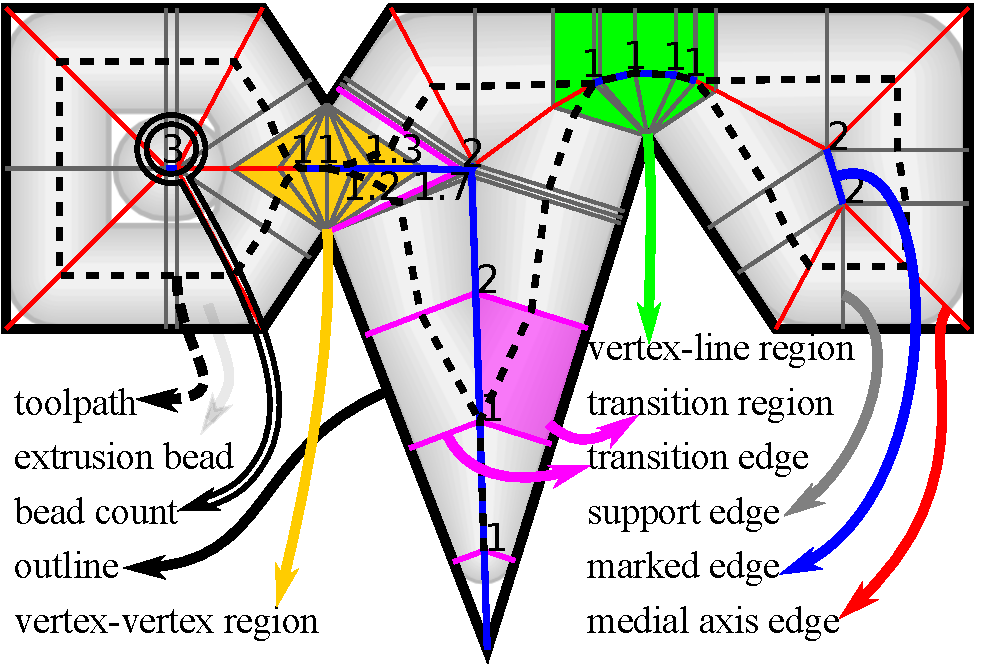
\includegraphics[width=.75\mycolumnwidth]{sources-method-legend2.pdf}
\caption{Illustrative explanation of terms and color coding that are consistently used in this paper.}
\label{legend}
\end{figure}




\Que{
What are the differences between the distributed and the inward scheme in Fig. 16(d) and (e)? Are they the same? 
}
\Ans{
We have adjusted the range of the inward distributed scheme to $N=2$ in order to generate a bigger difference between these images (Now Fig 18d and 18e).
The difference between inward and evenly distributed is now deemed to be so clear that the statistics graphs on the widths along the outer paths can be omitted.
}
\commits{735762b1e7daf31ae4465bf288ef867ded7da095 93352058a46fb391e323df16f45466adb8cad508
87b1b779b759a9ad115f3ea61243568bfa2e0cb6 % lil change in Fig 20 caption
ca322806c80ddc82c6f0c01d9ea5096b37ffcf8e % use smae rmin and N=2 in statistics
b4d03f0d8ea92ac9800794e154dc5b53e4448cab % don't compute graph for widths of outer bead
}
\paper{Beading schemes}
{
[See \cref{distributed_comparison}.]
}
\begin{figure}
\centering
\setlength{\figwidth}{.8\mycolumnwidth}
\setlength{\figheight}{.3\mycolumnwidth}
\begin{minipage}[b]{0.8\linewidth}
% -p test_geometry/wedge.svg -o wedge -s nrdi -n 1.5 -a --scale 1.5
\begin{subfigure}[t]{\figwidth}\centering
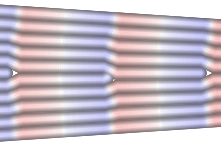
\includegraphics[width=\figwidth]{sources-validation-wedge-Distributed-pretty-evenly.png}
\caption{Evenly distributed}
\end{subfigure}
\begin{subfigure}[t]{\figwidth}\centering
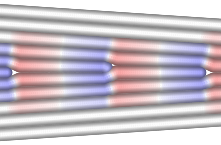
\includegraphics[width=\figwidth]{sources-validation-wedge-Distributed-pretty-inward.png}
\caption{Inward distributed}
\end{subfigure}
\end{minipage}
\begin{subfigure}[t]{.1\mycolumnwidth}\centering
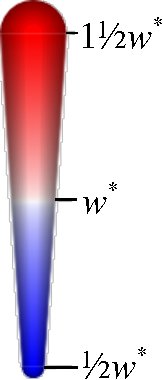
\includegraphics[height=\figheight]{sources-validation-widths-legend-small.pdf}
\end{subfigure}
\caption{
Closeup of toolpaths generated with the distributed \revise{}{and inward ($N=1.5$)} beading schemes for a large wedge shape.
Colors represent bead widths.
}
\label{distributed_comparison}
\end{figure}
\paper{Caption of Fig. 18}
{
\revise{}{In order to distinguish clearly from the Distributed scheme the Inward is limited to $N=2$.}
}
\paper{Caption of Fig. 20}
{
Visualization of the widths for the output toolpaths of the inward distributed beading scheme \revise{}{($N=3$) }applied to various example application objects.
}
\paper{5.2 Computational results}
{
Toolpaths of these 300 outline shapes are generated using the uniform technique as implemented by Clipper~\cite{johnson2014clipper} -- a state-of-the-art polygon offset library,
and by our framework using four beading schemes, i.e. the constant bead count scheme with a bead count of $C=4$, the centered, the evenly distributed, and the inward distributed beading scheme using \revise{$N=3$}{$N=2$}, all with a preferred bead width\revise{s}{} of \revise{$w^* = \SI{0.4}{\milli\meter}$}{$w^* = \SI{0.5}{\milli\meter}$ and using the widening meta-scheme to enforce a minimum printed feature size of $w_\text{min}=2r_\text{min}=\SI{0.3}{\milli\meter}$}.
}
\paper{5.2.2 Uniformity}
{
\revise{
We compared the width uniformity of the 6 outer beads for the inward and evenly distributed schemes, the distribution of these extrusion widths is shown in \cref{widthIndexedHistogram}. 
The outer beads of the inward distributed scheme deviate less from the preferred width compared to the evenly distributed scheme.
}{}
}



\Que{
In Fig. 17(b), where is the curve for the ”uniform” case?
}
\Ans{
We've added it back in.
Note that the width of the uniform case is \SI{0.4}{\milli\meter} \emph{everywhere}, so the curve is not really informative.
}
\commits{e5f3649455c73c8146e8d07cce13bc1e89d84cbb}


























\section{Reviewer 2}
\Summary{
The paper is generally well written with clear illustrations. 
}
\Ans{
Thank you.
}



\Que{
There are occasional omissions, perhaps unintentional, such as the definition of a skeleton - see section 3.1, second paragraph. 
}
\Ans{
Early in the overview section we don't have a mathematical definition of the term `skeleton' yet.
Seeing as there are multiple possible skeletonizations we use the term `skeleton' as an umbrella term and later give a specific definition of skeletons such as the Voronoi Diagram, the Medial axis and the trapezoidal skeletonization.
We have added a clarification in the overview section for the readers who don't know what the umbrella term would refer to.
}
\commits{
98af7981a67e9d54b3c47db5a2a41035e1278aeb % lil explanation of 'skeleton' (reviewer 2.1)
5356492b5a9a690228ffdb6a6a26cf10d099a7d4 % make clear that a skeleton is an undefined term (reviewer 2.1)
74227189eba03d13e18249f3235680691c6ebea9 % clarify skeleton more
}
\paper{3.1 Method overview}{
Our method starts with computing \revise{the skeleton of the input polygon}{a graph which represents the topology of the input polygon: its \emph{skeleton}. 
Our skeleton is} based on the medial axis transform (MAT), a strategy that has been commonly used for generating contour-parallel toolpaths~\cite{eiamsa2003toward}
}





\stepcounter{question}
\subQue{
The authors seem to use linear approximations of the medial axis - see Figure 2 (b), which is understandable given the fact that they compute the MA with the Boost library. If this is so, can the authors comment on the implications of this approximation?
}
\Ans{
We chose for linear approximations because they simplify the algorithms,
whereas we chose for Boost because it seemed more stable than alternative libraries.

The discretization is handled in section 3.2. Skeletal trapezoidation, second paragraph.
The discretization simplifies the algorithm, potentially at a slight computational cost.
Because we used $d^\text{discretization} = \SI{0.2}{\milli\meter}$, we can expect the discretized skeleton to deviate from the real skeleton by approximately \SI{0.013}{\milli\meter}, which is within the range of accuracy of the hardware system used.
The computation of this value is complicated by the fact that the discretization always introduces a sample point at the apex and at the boundaries of significant portions of the parabola.
(See section 3.3 Significance measure, last paragraph.)
See Figure~\ref{response_parabola_discretization}.
}
\commits{
64029a6ef57cf8044c521075ebc70cddfb52156b % mention 0.01mm in paper
}
\paper{3.2 Union of cones, Skeletal trapezoidation}
{
The vertex-line and vertex-vertex edges are discretized into pieces with a length up to \revise{$d^\text{discretization}$}{\SI{0.2}{\milli\meter}, which gives an approximation error of only $\pm$\SI{0.01}{\milli\meter}}.
}


\begin{figure}\centering
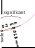
\includegraphics[width=.3\mycolumnwidth]{response_parabola_discretization}
\caption{Parabola discretization.
Thick black is part of the outline.
Red is significant skeleton, violet is non-significant skeleton.
}\label{response_parabola_discretization}
\end{figure}






\subQue{
For example, what happens if the obtuse outside angle in Figure 2 goes to 0? 
}
\Ans{
That figure is reproduced here in Fig.~\ref{overview_outline}.
As the rightmost two points move right, the degree of the corner in the middle goes to zero, which causes the parts of the parabola revealed to be more accurately described by the discretization than the highly curved part in the middle.
}
\begin{figure}\centering
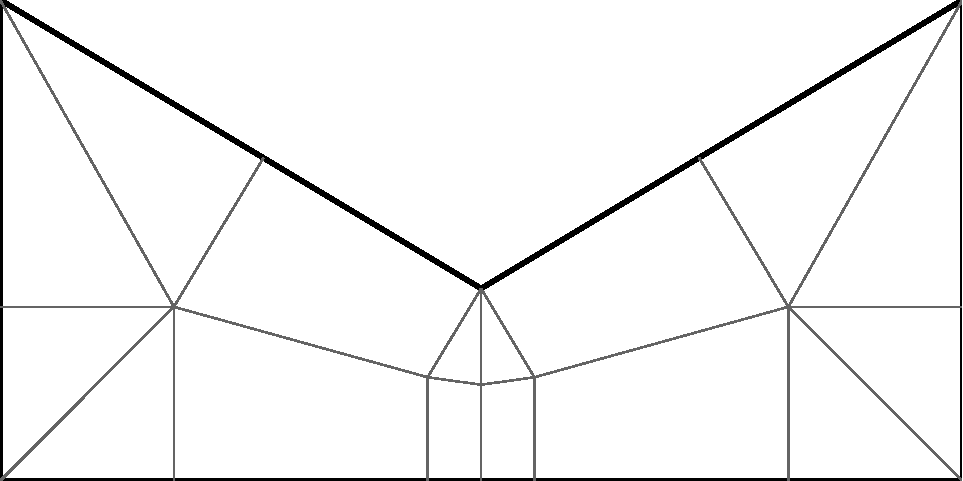
\includegraphics[width=.3\linewidth,rotate=-90]{response_simple_example_1}
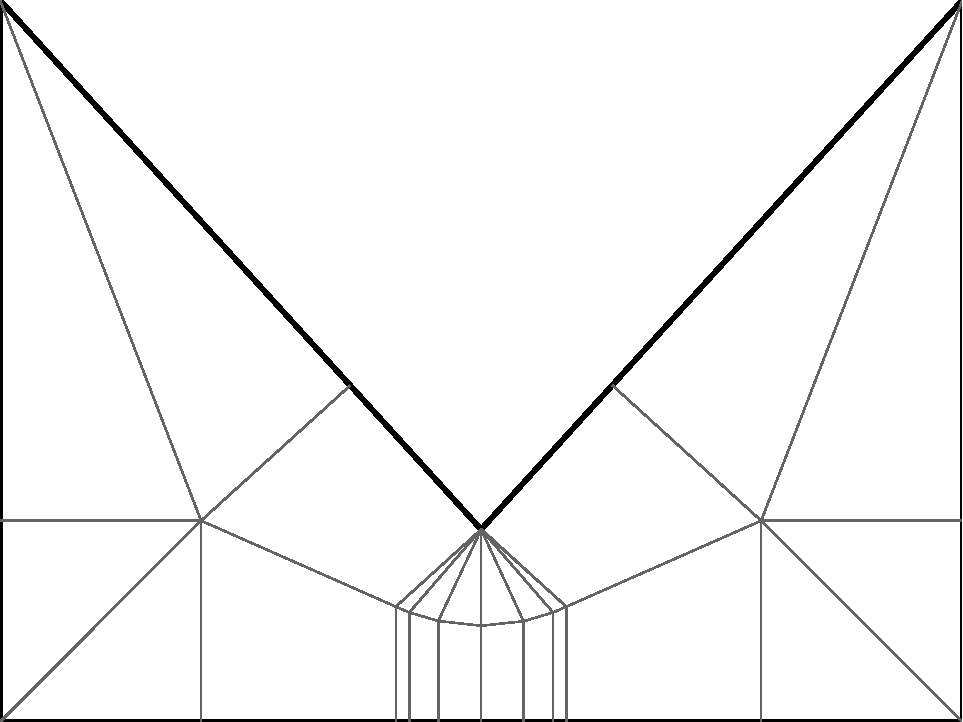
\includegraphics[width=.3\linewidth,rotate=-90]{response_simple_example_2}
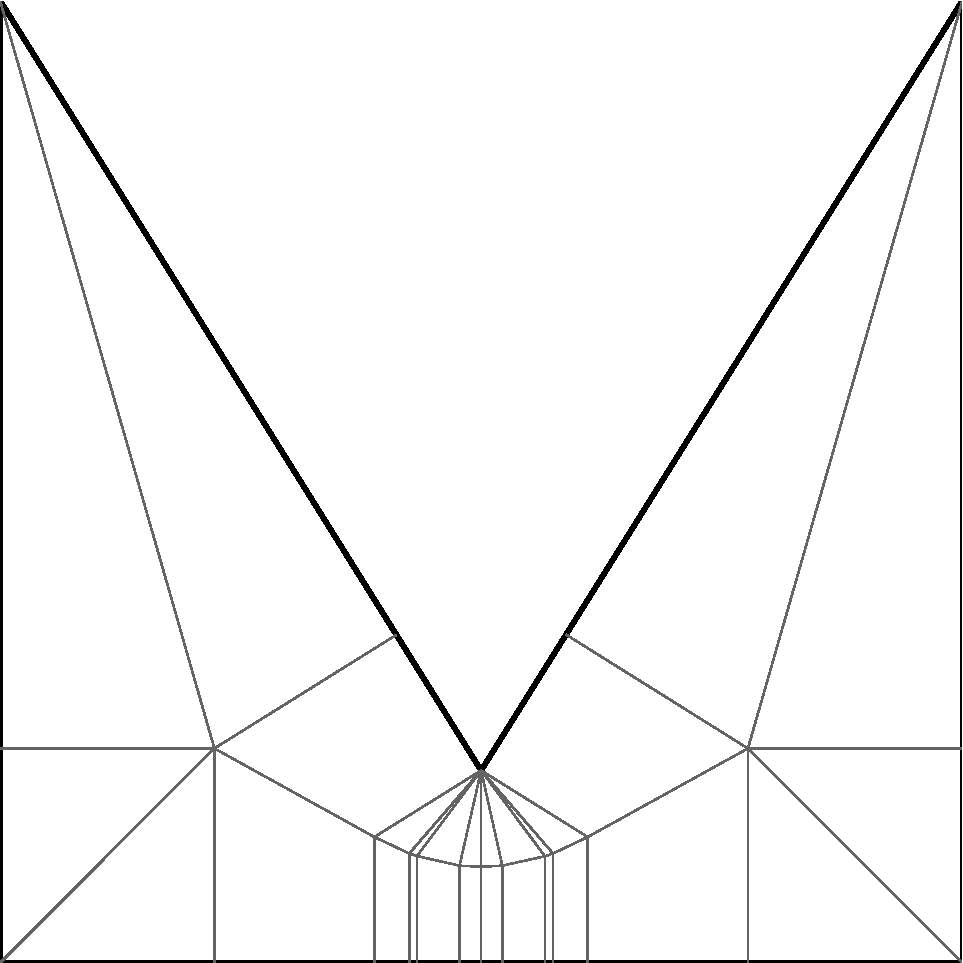
\includegraphics[width=.3\linewidth,rotate=-90]{response_simple_example_3}
\caption{Skeletal trapezoidation}\label{overview_outline}
\end{figure}









\Que{
As the authors correctly point out, the MA is not piecewise linear even for polygonal boundaries. In 3.2, second paragraph, the authors state that "the medial axis is a compact and complete representation of the shape". First, the MA + the radius function can be considered a shape representation, which is not true for the MA by itself. Second, the statement that the authors is meant to be generic, but it is not clear what compact means for a medial axis that is not piecewise linear. One can argue that the polygon itself is a rather compact representation of the shapes considered in this manuscript. 
}
\Ans{
Indeed the statement was meant generically, but we agree it lacked substance.
The wording is now changed to better describe the general role of the medial axis in research.
}
\commits{d3f19c04e3bb0d80c0b162531dbf576fc705d77c}
\paper{Medial axis transform}{
The medial axis is a \revise{compact and complete representation of}{representation commonly used to analyse} a shape.
}








\Que{
More generally, the technique seems to effectively be a variable offset scheme, but there is little discussion about what is known about variable offsets. 
}
\Ans{
Indeed the locations of the junctions in the toolpaths are at variable offsets from the outline, but that doesn't make our framework a variable offset scheme, because the junction locations are determined both by the radius in the central regions and the location of the outline.
Computing the same toolpaths using some variable offset scheme would still require the computation of the radial distances in central regions and relate those to outline locations, which means that we would still need to use the skeleton.
Therefore a variable offset scheme is not an alternative to our framework.

We have not found any variable offset scheme literature which is specifically on toolpath generation, so it wouldn't fit in the related work section.
The method section, however, doesn't go into variable offset schemes because offset schemes apply offset values given at the outline, while our framework principally relates the outline and the skeleton.
}



\Que{
Moreover, the proposed technique seems to rely on rather accurate control of the width w of the deposited material, but it is not clear whether such control is achievable in practice. 
}\label{s5_prints}
\Ans{
The proposed technique relies \emph{less} on the accuracy of the control than existing techniques – as exemplified by Fig 19d.

The photos of our print results already showed that adaptive width control is possible up to an admittedly insufficient extent.
We have developed a new method for actualizing adaptive width control which can readily be applied to unmodified FDM systems such as the Ultimaker S5: \emph{back pressure compensation}.
We show the results of back pressure compensation in a separate figure which clearly shows the achieved variance in bead width.

All paragraphs on the physical realization have been put together and moved to after the theoretical analysis:
we moved the section on limitations of linear advance algorithms (5.5 Discussion on implications) together with the section on Printing results to after the comparison of beading schemes (now 5.2).
}
\commits{
%3d7238e2787f17c4cff63804eb4b84439ff85f1b  % initial printing results section 5.2
%b5abdd980240cd4ca964ed0f4751c207baa09b85 % move 5.5 to 5.2
a0e98d1079b3ab3b262908ea056939813fc49c73 % move 5.2 to 5.3 and overhaul
6362bb7f1ff11e15efc6667fc7863ca12a29a8a9 % mention in intro and conclusion
22cb3664ddc722d25e0a73df905100410f8ebf10 444a00a54100e402024335b79265b6900017bc1d ab38e07c84b6e62dc028d224b7a57bba9239552f cb3325a9cf00457fab5f1bdc5d29f1d178de4e35% S5 prints
d375878a8a6d01c53436aeb9c473dbedd8f3edcf % prints discussion
125162ad9878c0fb5a054f1bab34aa7b1353b86c % better var width test figure
34e923fbf4c2ad45bf2dd0a03ef70d4a714b4b0b % lil comma (x2)
1b7bb61648b97b8084ca8817aa457bde2c91e1b3 % lil: explain unexplained math symbol 
}
\paper{5.2 Printing results}
{
\revisepar{
Test prints were performed on a custom FDM hardware setup, with a standard \SI{0.4}{\milli\meter} nozzle and a filament extrusion drive directly mounted on the print head.
The firmware of the printer employs \emph{linear advance} for accurately realizing adaptive deposition width:
gaining the extra pressure required to change to a wider bead is realized by 'advancing' an extra amount of filament into the physical system~\cite{tronvoll2019investigating}.
We set the preferred width to $w^* = \SI{0.6}{\milli\meter}$, to avoid fluttered printing of lines narrower than the nozzle size.
We used a layer thickness of \SI{0.2}{\milli\meter} and a movement speed of \SI{10}{\milli\meter\per\second}.
}{}

\revisepar{
The prints are shown in \cref{prints_old}.
Because of inaccuracies in the deposition control system some of the prints show defects.
Such defects are less prevalent for the inward distributed beading scheme than the other schemes.
The prints which employ the uniform offsets technique show a lot of underfill, which impacts the visual quality of the print.
Moreover, in the case of the regular honeycomb there are several fully disconnected hexagons, which means the object falls apart.
The difference between the centered and the inward distributed schemes is less pronounced.
We can still see some loosely connected extrusion segments in both, which is attributable to inaccuracies in the extrusion system.
However, the middle of \cref{wedge_print} exhibits more defects in the regions where the centered scheme produces extreme bead widths.
The bottom print shows that the inward distributed beading scheme produces smoother prints with less defects.
}{}

\begin{figure}
\centering
\begin{subfigure}{\mycolumnwidth}\centering
\setlength{\figwidth}{\mycolumnwidth}
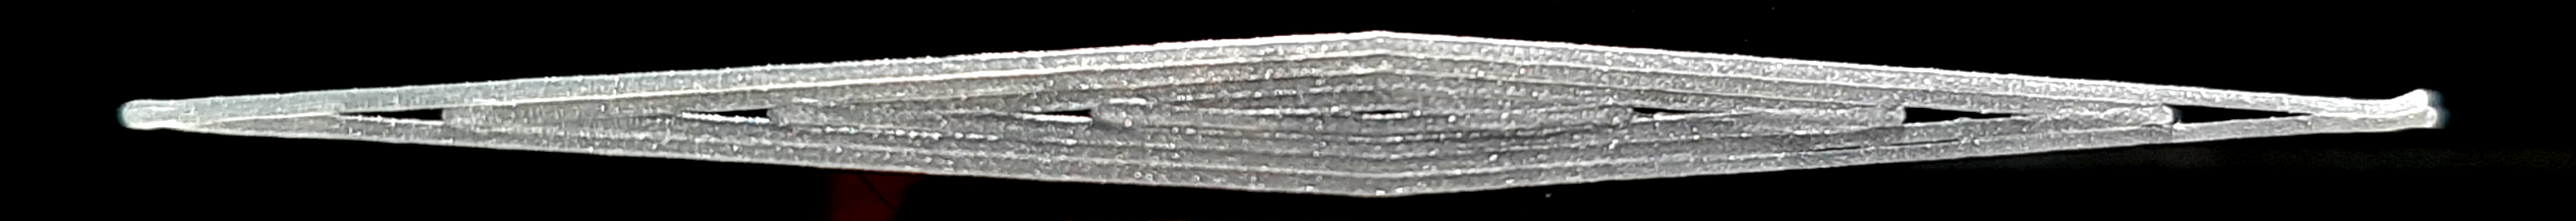
\includegraphics[width=\figwidth]{sources-applications-P3-print-wedge-naive-edited.png}
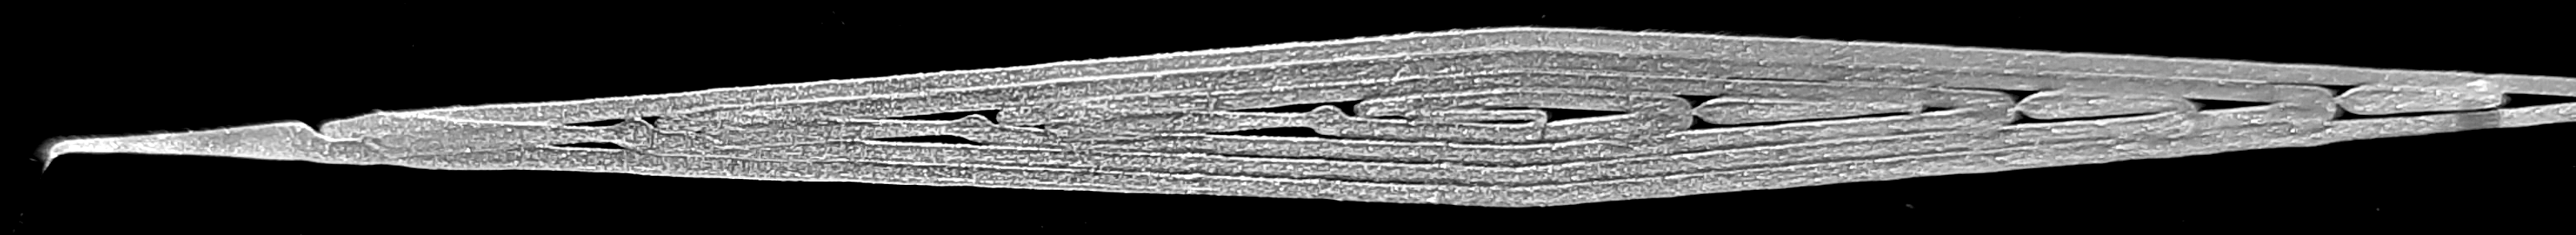
\includegraphics[width=\figwidth]{sources-applications-P3-print-wedge-center-edited.png}
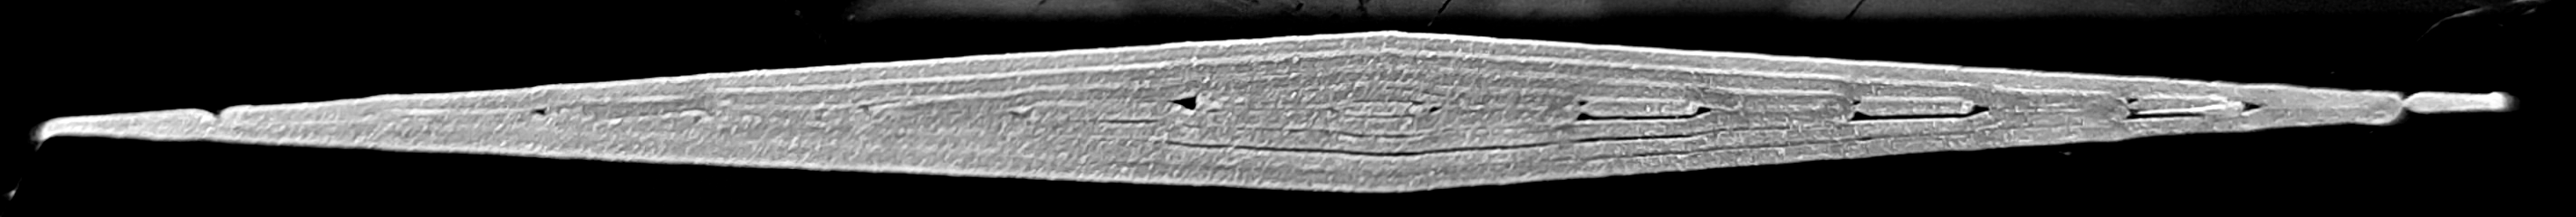
\includegraphics[width=\figwidth]{sources-applications-P3-print-wedge-inward-edited.png}
\caption{Uniform (top), centered (mid) and inward distributed (bottom)}\label{wedge_print}
\end{subfigure}
\setlength{\figheight}{.38\mycolumnwidth}
\setlength{\figheightTwo}{.47\mycolumnwidth}
\setlength{\figwidth}{0.32\mycolumnwidth}
\begin{subfigure}{\figwidth}\centering
%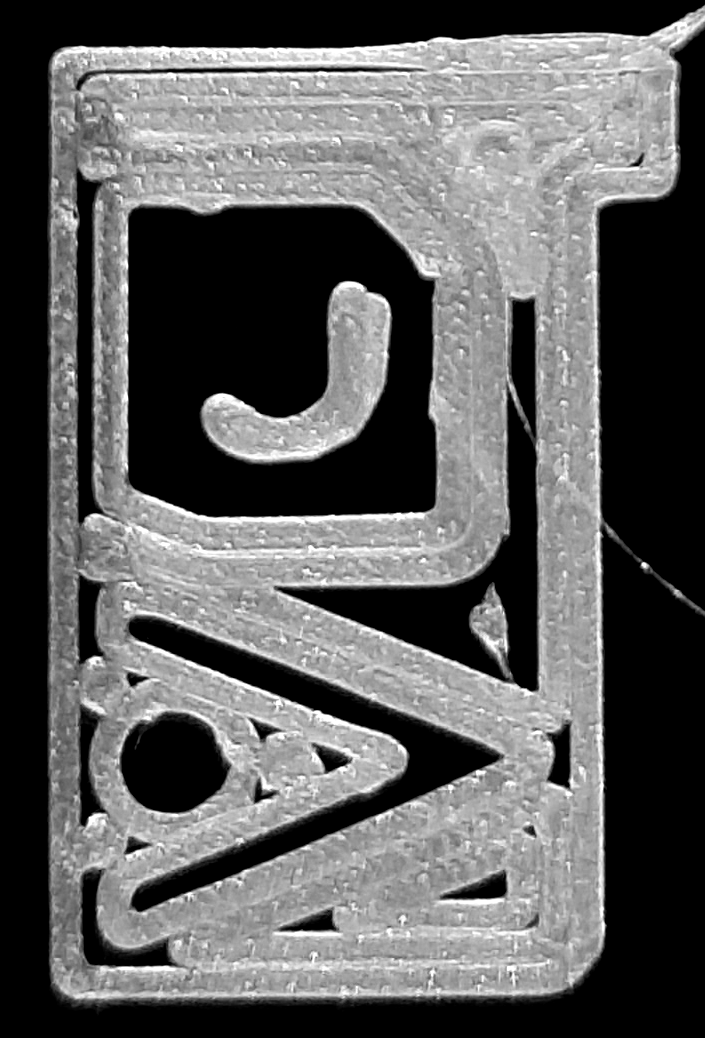
\includegraphics[height=\figheightTwo]{sources-applications-gMAT-naive.png}
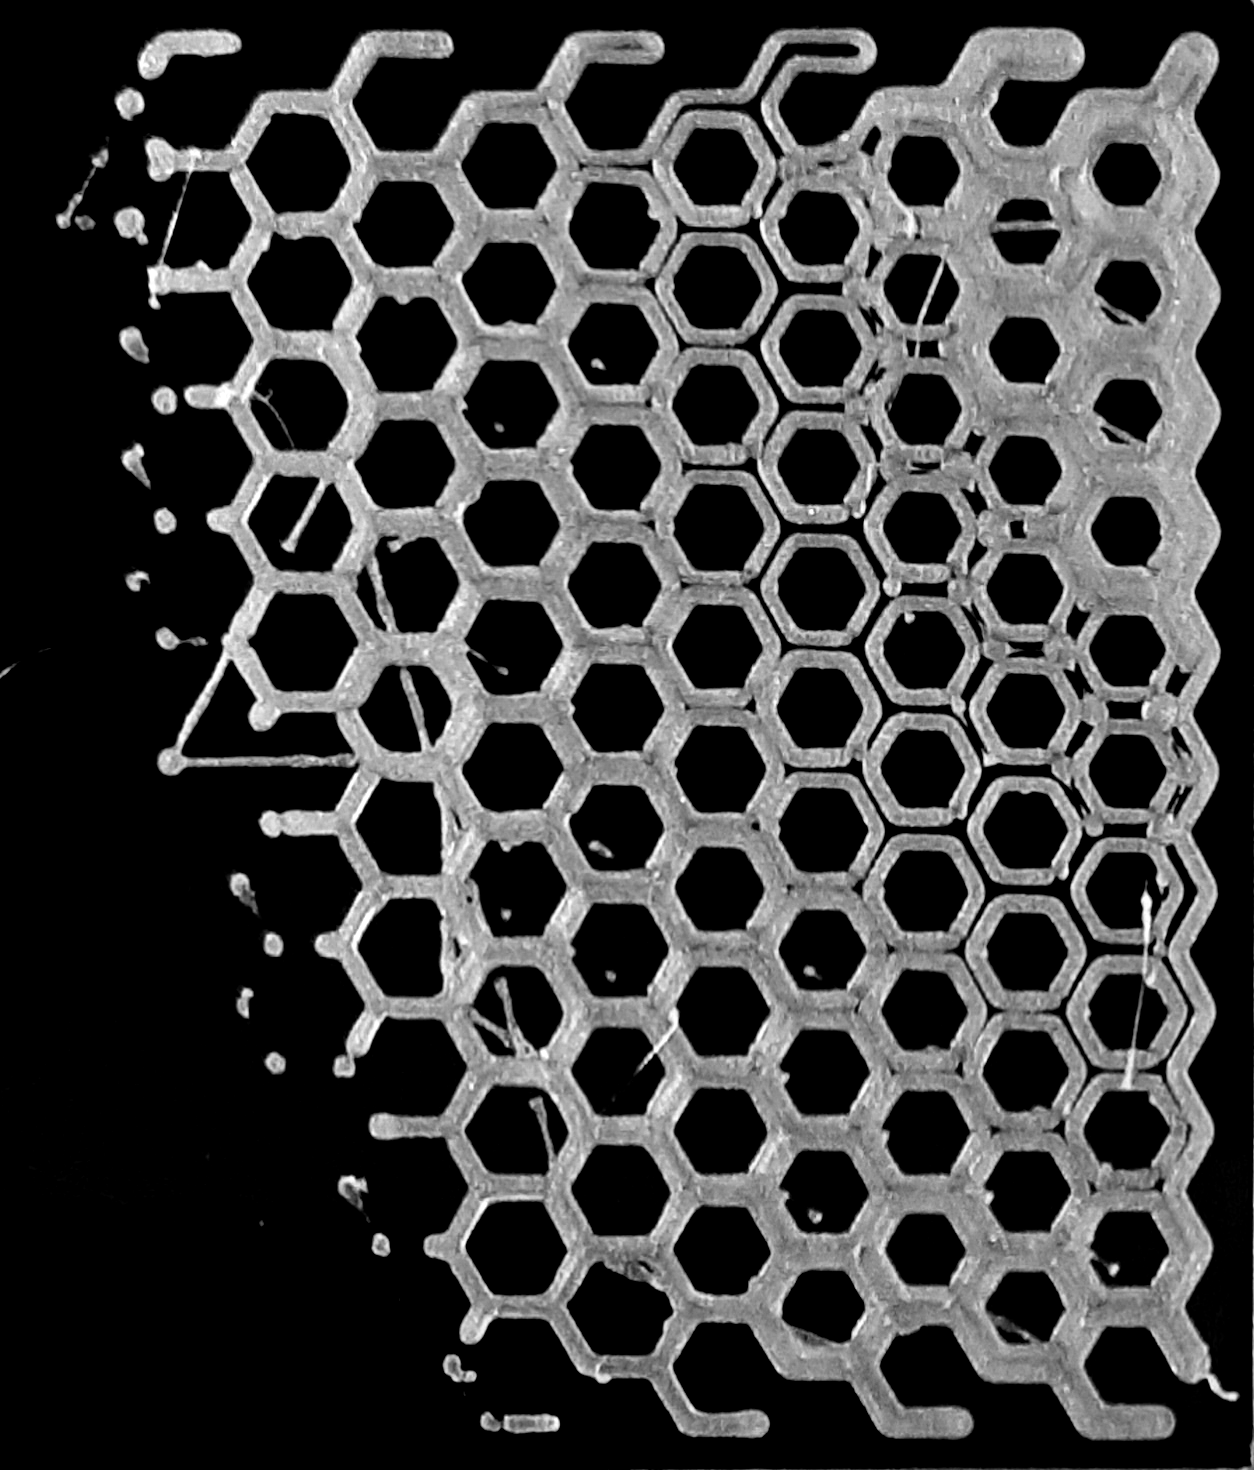
\includegraphics[height=\figheight]{sources-applications-P3-print-hex-naive-edited.png}

\includegraphics[width=\figwidth]{sources-applications-P3-print-UM-naive-edited.png}
\caption{Uniform}\label{print_naive}
\end{subfigure}
\begin{subfigure}{\figwidth}\centering
%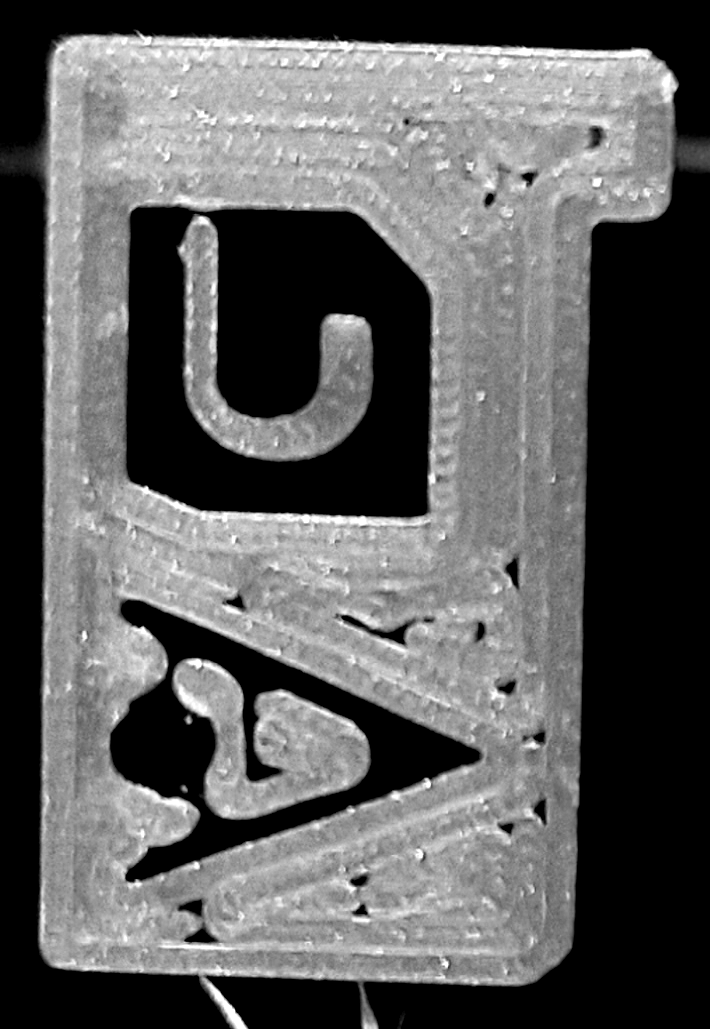
\includegraphics[height=\figheightTwo]{sources-applications-gMAT-center.png}
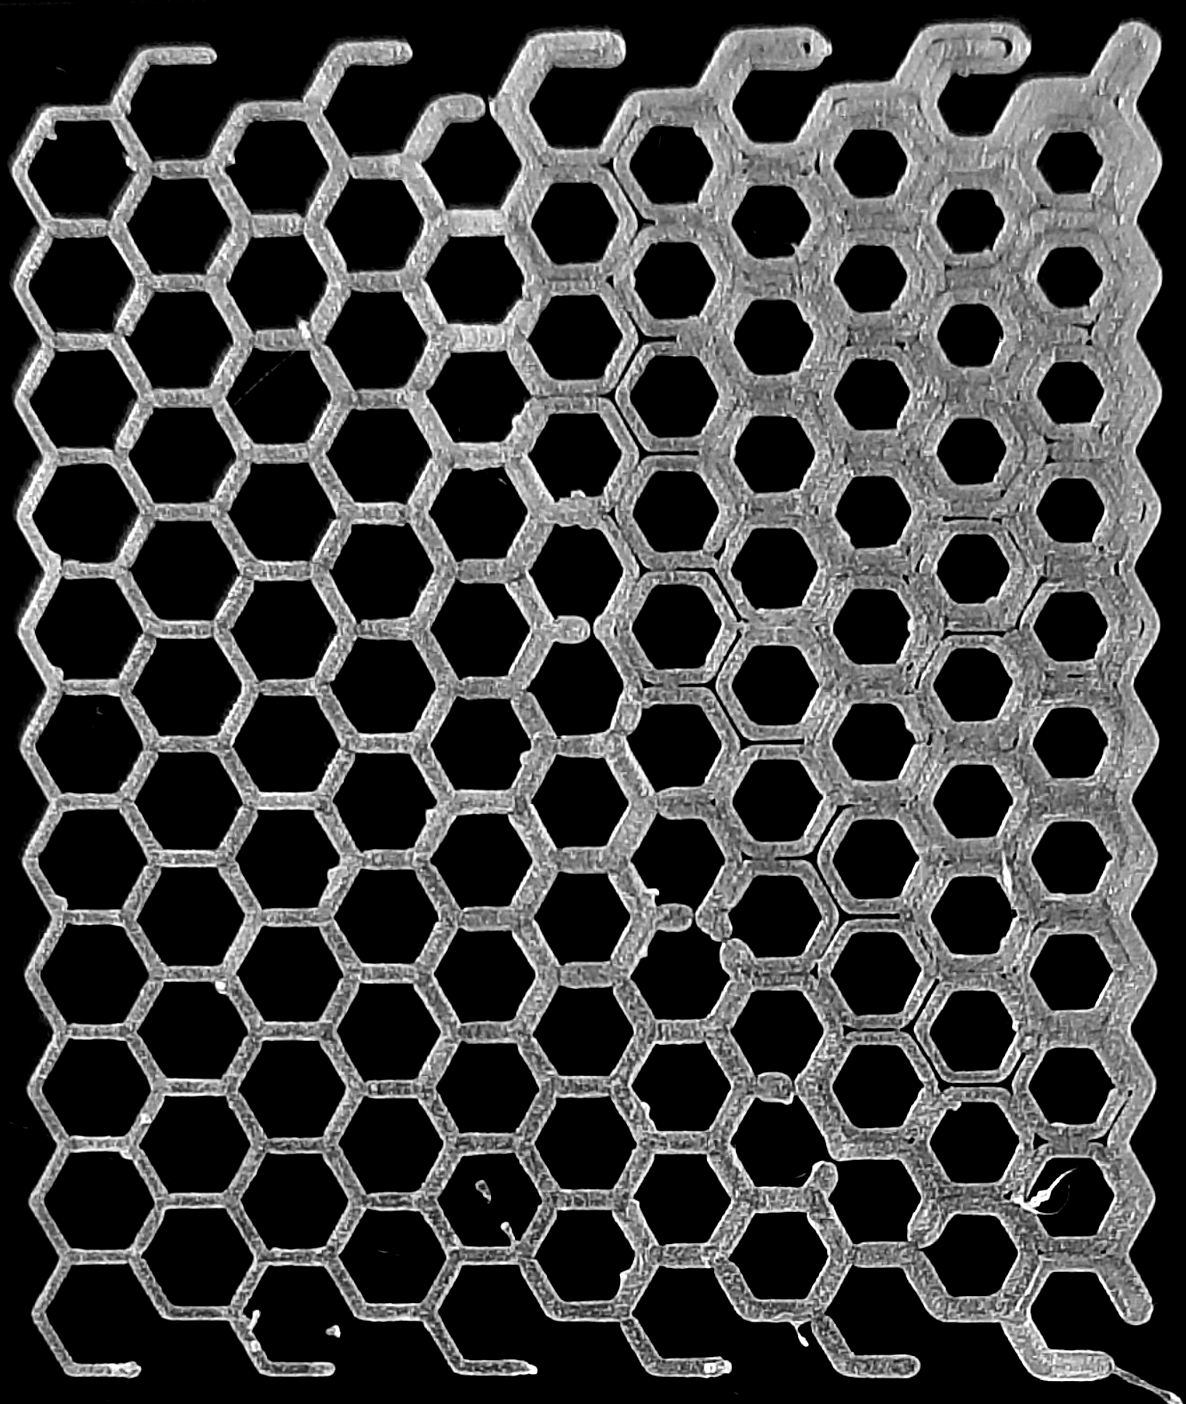
\includegraphics[height=\figheight]{sources-applications-P3-print-hex-center-edited.png}

\includegraphics[width=\figwidth]{sources-applications-P3-print-UM-center-edited.png}
\caption{Centered}\label{print_center}
\end{subfigure}
\begin{subfigure}{\figwidth}\centering
%\includegraphics[height=\figheightTwo]{sources-applications-gMAT-inward.png}
\includegraphics[height=\figheight]{sources-applications-P3-print-hex-inward-edited.png}
\includegraphics[width=\figwidth]{sources-applications-P3-print-UM-inward-edited.png}
\caption{Inward distributed}\label{print_inward}
\end{subfigure}
\caption{
Test shapes printed using the uniform scheme, centered scheme and the inward distributed scheme.
The uniform technique produces distinct underfill areas.
The centered scheme shows some defects due to inaccurate control of extreme deposition widths.
The inward distributed scheme produces the least defects.
}
\label{prints_old}
\end{figure}

\revisepar{}{
\subsection{Fabrication}
In order to accurately manufacture adaptive width toolpaths using an off-the-shelf 3D printing system,
we need a model which relates the required width to process parameters such as movement speed and filament extrusion speed.
A different approach might be appropriate depending on whether the filament feeder is mounted directly on the print head (a.k.a. \emph{direct drive}) or the filament fed from the back of the printer to the print head via a \emph{Bowden tube}.
Because Bowden style 3D printing systems have the filament feeder relatively far away from the nozzle, changing the internal pressure in the system requires a large amount of filament movement, which requires a prohibitive amount of time.
}

\revisepar{}{
\subsubsection{Back pressure compensation}
We therefore keep the internal pressure constant, and vary the movement speed instead.
%In order to accurately realize a varying bead width we vary the movement speed, while keeping the internal pressure in the system constant.
One approach would be keep the filament inflow $f$ (in \si{\milli\meter\cubed\per\second}) constant by varying movement speed accordingly \cite{Kuipers2018}.
However, that doesn't result in the intended filament outflow variation - see \cref{zero_back_pressure}.
We conjecture that the filament outflow is related to the total pressure in the system,
which depends not only on the amount of filament in between the feeder wheel and the nozzle (which we keep constant), 
but also depends on the back pressure that the previous layer exerts on the filament protruding from the nozzle.
We conjecture that the amount of back pressure is monotonically related to the requested line width and compensate for the back pressure using a simple linear model:
}

\revisepar{}{
\begin{align}
 v(w) &= \frac{f(w)}{h w} \\ 
% f &\sim p \\
% p &= p_\text{in} + p_\text{ext} \\
% p_\text{in} &= C \\
% p_\text{ext} &\sim w \\
% p_\text{ext} &= w / w^* - 1 \\
% f &= f^* - k p_\text{ext} \\
 f(w) &= f_0 - k \left( w / w_0 - 1 \right)
 % f_0 &= v_0 w_0 h 
% v &= \frac{f^* - k p_\text{ext}}{h w} \\ 
% v &= \frac{v^* w^* h - k (w / w^* - 1)}{h w}
\end{align}
where
$v(w)$ is the movement speed as a function of requested bead width $w$,
$f(w)$ is the filament outflow,
$f_0$ is a constant reference flow,
$w_0$ is a constant reference bead width
and
$k$ is the amount of back pressure compensation.
}

\revisepar{}{
% adapted from 5.5 Discussion on implications
% limitations of back pressure compensation
Our back pressure compensation method effectively changes the speed to realize adaptive width,
but this approach is limited, since the movement speed is constrained by acceleration considerations near bends in the toolpath~\cite{Ertay2018}.
Moreover, as the layer height is decreased the back pressure becomes larger compared to the internal pressure, which might cause the back pressure compensation method to demand prohibitively slow movement speeds.
Furthermore, the shape and filling of the previous layer might influence the amount of back pressure.
%
% direct drive & pressure advance
Accurate flow control can be further enhanced by using a direct drive hardware system and by employing \emph{pressure advance algorithms} which dynamically change the internal pressure \cite{tronvoll2019investigating}.
Conversely such a setup might benefit from some form of back pressure compensation as well.
}

\revisepar{}{
\subsubsection{Print results}
Using increments of $0.1$ we established that using a factor of $k=1.1$ yields satisfactory bead width variation for our setup where we use
$f_0 = v_0 w_0 h $
with
$v_0=\SI{30}{\milli\meter\per\second}$, 
$w_0=\SI{0.4}{\milli\meter}$
and
$h=\SI{0.1}{\milli\meter}$.
See \cref{back_pressure}.
The fact that the printed lines are wider than intended is compensated for using a flow reduction to \SI{90}{\percent}.
%
Test prints were performed on an unmodified Ultimaker S5 system,
with a standard  \SI{0.4}{\milli\meter} nozzle
and PLA filament.
The printing order is determined greedily by choosing the closest point of a polygonal extrusion path, or the closest of either end point in case of an open polyline extrusion path.
Because the machine instructions file format \emph{G-code} doesn't natively support adaptive width beads,
we discretize adaptive width extrusions into \SI{0.2}{\milli\meter} long segments of the average width.
The results can be viewed in \cref{prints}.
}

\begin{figure}
\centering
\setlength{\figwidth}{0.32\mycolumnwidth}
\setlength{\figheight}{0.5\mycolumnwidth}
\begin{subfigure}[t]{\figwidth}\centering
\includegraphics[angle=90,height=\figheight]{sources-validation-backpressure_0_0}
\caption{$k=0$}\label{zero_back_pressure}
\end{subfigure}
\begin{subfigure}[t]{\figwidth}\centering
\includegraphics[angle=90,height=\figheight]{sources-validation-backpressure_1_1}
\caption{$k=1.1$}\label{back_pressure}
\end{subfigure}
\begin{subfigure}[t]{\figwidth}\centering
\includegraphics[angle=90,height=\figheight]{sources-validation-backpressure_2_0}
\caption{$k=2.0$}\label{too_much_back_pressure}
\end{subfigure}
\caption{
Print results (black) of the varying width test on top of a dense white raft.
Target widths in green.
\subref{zero_back_pressure} Simple flow equalization without back pressure compensation results in nearly constant bead widths.
\subref{back_pressure} A value of $k=1.1$ seems to produce good results.
}
\label{back_pressure_compensation}
\end{figure}

\revisepar{}{
% discussion of print results
In \cref{print_naive} the underfill problem of the naive uniform offset approach is most prevalent for the Ultimaker word mark, which negatively impacts the visual quality and the stiffness of the part.
Moreover, in the case of the spatially graded honeycomb there are several fully disconnected hexagons, which means the object falls apart when picked up.
The honeycomb print is also missing all parts which are slightly more thin than the preferred bead width $w^*$.
\Cref{print_center} still shows some underfill, but considerably less than the uniform approach.
These prints also exhibit dark regions where the translucency of the layer is less because the bead is higher.
This can be explained by inaccuracies in the back pressure compensation method, which arise for bead widths which deviate from the preferred width by a large amount.
\Cref{print_inward} diminishes the underfill nearly completely and the visual quality of these prints is more homogenous than those of the other methods.
Moreover, the absence of dark regions signifies that our proposed method is more robust against inaccuracies in the deposition system.
However, both the centered and inward distributed approach introduce transitions to a different bead count in the word `Delft', which reduces the dimensional accuracy on the outline around those locations.
}

\revisepar{}{
\begin{figure}
\centering
\setlength{\figwidth}{\mycolumnwidth}
\begin{subfigure}{\figwidth}\centering
\includegraphics[width=\figwidth]{sources-applications-result-prints-target}
\caption{Outlines}\label{print_outlines}
\end{subfigure}
\begin{subfigure}{\figwidth}\centering
\includegraphics[width=\figwidth]{sources-applications-result-prints-naive-bw.png}
\caption{Uniform}\label{print_naive}
\end{subfigure}
\begin{subfigure}{\figwidth}\centering
\includegraphics[width=\figwidth]{sources-applications-result-prints-center-bw.png}
\caption{Centered}\label{print_center}
\end{subfigure}
\begin{subfigure}{\figwidth}\centering
\includegraphics[width=\figwidth]{sources-applications-result-prints-inward-bw.png}
\caption{Inward distributed}\label{print_inward}
\end{subfigure}
\caption{
Test shapes printed using the uniform scheme, centered scheme and the inward distributed scheme.
The uniform technique produces distinct underfill areas.
The centered scheme shows some defects due to inaccurate control of extreme deposition widths.
The inward distributed scheme produces the least defects.
}
\label{prints}
\end{figure}
}

\revisepar{
\subsection{Discussion on implications}
Note that the current industry standard in FDM printing employs little to no bead width variation.
Properly performing bead width variation calls for adaptations and developments in printers and firmware.
In the beading schemes we set a transition length of $t(n) = w^*$.
That will demand changes in cross-sectional area of the bead up to \SI{200}{\percent} over a small distance that is comparable to the nozzle size, which is challenging for some hardware systems.
Varying the movement speed can be utilized to change the cross-sectional area, but this approach is limited, since the movement speed is constrained by acceleration considerations near bends in the toolpath~\cite{Ertay2018,Kuipers2018}.
Our schemes require a more accurate control of the volumetric flow rate in \si{\milli\meter\cubed\per\second}.
Using a filament feeder directly mounted on the print head (a.k.a. direct drive) can control the flow more dynamicaly then FDM printers where the material is fed through a Bowden tube from a feeder mounted on the frame.
Still direct drive printers require some control system in order to accurately change the volumetric flow rate such as pressure advance algorithms~\cite{tronvoll2019investigating}.
Yet inaccuracies in direct drive systems employing advance algorithms might arise due to the changes in back-pressure required by changing bead size.
We expect that developments in printing hardware and firmware will address these challenges in the future.
}{}

\revisepar{
Another limiting factor for adopting adaptive bead width is the format of G-code which stores machine instructions.
G-code does not support moves with varying cross-sectional area.
A typical extrusion move \lstinline!G1 X$x$ Y$y$ E$v$! only specifies the total amount of volume $v$ to be extruded in the move, not how that total amount should be distributed along the extrusion move.
A workaround is to approximate a variable width extrusion segment by smaller segments with constant width.
However, this introduces errors nevertheless.
Ideally the G-code language would be expanded in some way to allow for extrusion segments with varying cross-sectional area.
}{}
}




\Que{
At the same time, the scheme can potentially result in trajectories with many inflection points - this is slow and demanding for the machine. 
}
\Ans{
We have added statistics on fabrication time and discussed our findings.
See our response to 1.3.
}





\Que{
Finally, the examples provided depict the results obtained by the authors by "emulating" other techniques, but not with the actual results produced by the other techniques. While the reason behind this choice is easy to guess, it weakens the effectiveness of the claims. Adding careful discussions/extensions to support these questions would make the paper stronger.
}
\Ans{
We've added a paragraph to section 5.3. Limitations, which discusses these emulation limitations.
}
\commits{
639dccad8e97fa1f0bdbb28e16b64f587572792d % paragraph in limitations
}
\paper{5.3 Limitations}
{
\revise{}{
Finally it should be noted that although our framework can accurately emulate the constant bead count approach by \citeauthor{Ding2016a}, its emulation of the centered approach by \citeauthor{Jin2017JMS} is imperfect.
The transitions resulting from out framework introduce sharper corners and there is more width variation in those corners.
Whereas the width of the connecting segment in the approach by \citeauthor{Jin2017JMS} is the preferred width $w^*$, the bead widths closer to the center resulting from our framework will be twice the local radius, which is larger than $w^*$.
However, this inflated bead width variation is expected to have an insignificant impact on the measured bead width variation.
}
}








\section{Reviewer 3}
\Summary{
Paper is well written. It is mostly easy to follow but overall, I find the the contributions somewhat incremental and the motivation not convincing. The paper mostly feels like a technical report. I am not sure if the methods overall teach enough to the researchers in the field to open up new research possibilities. My specific comments are below: 
}
\Ans{
Thank you for your feedback.

}




\Que{
The title is a little misleading that the presented approach may be used for general “Additive Manufacturing”. However, my understanding from the text is that it is designed particularly for FDM. I believe it is important to highlight this in the title. Otherwise, there should be enough evidence to prove that it can be applied to other kinds of printing processes, such as SLS, SLA, DMLS etc. 
}
\Ans{
The title has changed.
}
\commits{
64eb2f2c1cbb28258a984b5f84ea6e3a039ee1f0
1935689874235a6c1d5b8f0fed725afa53804935 % don't introduce only one strategy for FDM only
}
\paper{Title}{
A framework for adaptive width control of dense contour-parallel toolpaths in \revise{additive manufacturing}{fused deposition modeling}
}
\paper{Introduction, bulletlist}{
A specific beading scheme \revise{for FDM printing}{} which [\dots]
}





\Que{
It would be nice to discuss why contour-parallel toolpaths are needed or selected. In what situations, these are required as opposed to zigzag style (or direction-parallel as referred in the text) patterns. Without such a discussion, the motivation seems a little weak. In the second paragraph of introduction, there is a short discussion about this but it sounds like the authors assume that even the perimeters (or outline) are printed with direction-parallel extrusion. However, common approach in FDM is to print the perimeters with contour parallel toolpaths and fill the inner region with direction-parallel paths only (as later acknowledged in the related work 3rd paragraph). I think the motivation for contour parallel toolpaths needs to be justified further. 
}
\Ans{
The industry standard is to use a combination of contour-parallel and direction-parallel.
We now clarify why contour-parallel is (partly) used and that in as much as contour-parallel is used, our approach improves on the industry standard.
We have also developed and presented a new meta-scheme for generating only a limited number of perimeters, which shows that our technique is compatible with the industry standard for FDM 3D printing.
See also the changes to the paper presented under question~\ref{widening_question}.
}

\commits{
6b0f8c78d31bd0c6946885da96f73f1cfc1a21ae % clarify widespread use of concentric toolpaths in abstract (reviewer 3.9)
ac800628951417dcb28bd6e3a0ed08801735acf4 % emphasize importance of contour-parallel toolpaths (reviewer 3.2)
a88ccd3309aef1233ed00ce9f22b244fe64668f4 % introduce shell meta-scheme and replace widening figure with widening+shell figure 
077c8ee138bb311a8ba9abf303af4b09e973637a % improve introduction of contour-parallel (reviewer 3.2)
8a11aa0105d1c7f1f5690c8e1f932be85a90bcae % more changes to shell + widening fig
}
\paper{Abstract}{
\revise{By densely filling consecutive 2D layers with contour-parallel extrusion toolpaths, FDM can produce parts with high stiffness and strength.}
{High stiffness parts are produced by filling the 2D polygons of consecutive layers (partly) with contour-parallel extrusion toolpaths.}
}

\paper{Intro}{
\revise{
Contour-parallel extrusion therefore leads to a less bumpy outline shape than direction-parallel extrusion does.
}{
Because contour-parallel extrusion leads to a more accurate outline shape it is common practice to print either the whole layer or only a limited number of outer perimeters that way.
This paper improves on those contour-parallel toolpaths and addresses several issues which commonly occur in 3D models with narrow geometry.
}
}



\Que{
Related work acknowledges the previous work sufficiently. However, the differences between the state of the art and the presented work are not clear. More discussion on where this work stands with respect to the state of the art is required. 
}
\Ans{
We have tried to address this in response to several other reviewers' comments.
See our response to question~\ref{difference_to_jin} and question~\ref{contributions}.
We now clearly claim that our method produces a lower range of bead widths than the state-of-the-art.
See also our response to question~\ref{widening_question} for clarification in the difference between Fig 1b and 1c.
}
\commits{
004894210fbc961f82b792fc702d1b67a1a8e8e8 lil lang improvement (reviewer 3.3)
9ac2c005c2eb1c0696e2582963353b038fa71072 use limited distributed strategy in fig 1 (reviewer 1.6, 3.3)
}
\paper{Fig 1}{
\subref{intro_wedge_distributed} Our approach minimizes over- and underfill with \revise{beads close to the nozzle size}{less extreme widths}.
}






\Que{
Isn’t it possible to put bounds on the width in the existing methods, such as the approach described in [9]? More discussion on that would be helpful. 
}
\Ans{
The bead width in Jin et al. is limited to $0.5 w^*$ to $1.8 w^*$ , which means the variation is a factor of $3.6$;
this was already described in the related work section, but the factor was wrongly said to be $2$ instead of $3.6$.
We emphasized that our method results in a bead width variation of $2$, rather than $3.6$ in the related work section and in the discussion section.
This factor comes from the transition from a single bead to two beads.
(The transition from zero beads to one is disregarded; it is controlled separately by the Widening meta-scheme.)
}
\commits{
661d8f6766548c287cb174070432097e396d198f 
92217c04e118dcf6f65b16a1ffcdfa40b4d50c0d give bounds on width variation (reviewer 3.4)
2f230ea9f26f9870027e80db89eae8774f19d339 fix bounds of width variation in Jin (reviewer 3.4)
acf8bbed0e530a3038d6fea064c33e7df6f0f933 % deviation > variation
}
\paper{Intro}{
The current \revise{state-of-the-art}{state of the art} for FDM printing developed by \citeauthor{Jin2017JMS} employs a strategy which alters the widths of the centermost beads \revise{at most by a factor of $2$}{within a range of widths with a factor of $3.6$}~\cite{Jin2017JMS},
}
\paper{3.4. Central height adjustment, Transition anchors, filtering paragraph}
{
\revise{}{This means that for some small regions we generate toolpaths with bead widths outside the typical range.}
}
\paper{5.2 Comparison of beading schemes, paragraph 3, 4}{
In \cref{TEST_Center_accuracy} we can see that
the centered beading scheme \revise{effectively }{}deals with both overfill and underfill and produces desired bead widths in all locations, except for the extrusion paths in the center, where the bead widths \revise{are within a factor 2 off from the desired bead width.}{range between $0.5 w^*$ and $1.8w^*$, i.e. the variation is within a factor of $3.6$.}

[\dots]

\revise{}{Moreover, because the quantization operator rounds to the nearest number of beads, in the worst case where we switch from a single to two beads the widths switch from $0.75w^*$ to $1.5w^*$, i.e. the variation is within a factor $2$, which is considerably lower the than factor of $3.6$ in the centered scheme.}
We therefore conclude that the distributed schemes \revise{result in bead widths closer to the preferred widths}{exhibit a lower bead width variation} compared to the centered scheme.
}






\Que{
Figure 4 and corresponding explanation in Section 3.2 are confusing. Why such decomposition is needed is not clear to me. 
}
\Ans{
Fig. 4 shows a legend of terms and color coding scheme used throughout the paper;
it doesn't show a decomposition.
It is unclear to us what this review comment is asking for.
}







\Que{
In Figure 3, why some of the edges in (c) (the ones in the center area) disappear in (d)?
}
\Ans{
Fixed. Fig 3 c and d now have the same discretization.
}
\commits{43cadb352a6a276bbaaab53f9b5b217bec4b3a2e}





\Que{
It is unclear how some of the parameters are adjusted, such as $\alpha_\text{max}, d_\text{max}^\text{unmarked}, d_\text{transition}^\text{max}, t_\text{beading}, d_\text{intersection}^\text{max}$. What are their effects on the end result? Selections seem somewhat arbitrary. 
}
\Ans{
We feel that some of the confusion was due to the fact that the chosen values for these variables is stated in a location in the paper far away from where they were introduced.
We now mention their value where they are introduced and explain their value further where needed.
Making these framework parameters independent of the beading schemes simplifies the definition of a beading scheme and greatly simplifies section 4. Beading schemes.
}
\commits{
64029a6ef57cf8044c521075ebc70cddfb52156b % d^discretization
1ea800d0b4f68963befff90e535d5c82748df5e2 % big rework
1c1159c482047f9aaa110e9086f800977adde268 % lil rephrase
}
\paper{3.2 Union of cones, Skeletal trapezoidation}
{
The vertex-line and vertex-vertex edges are discretized into pieces with a length up to \revise{$d^\text{discretization}$}{\SI{0.2}{\milli\meter}, which gives an approximation error of only $\pm$\SI{0.01}{\milli\meter}}.
}
\paper{3.3 Center classification, Significance measure}
{
\revise{}{A too large $\alpha_\text{max}$ may leave a lot of under-/overfill, while a too small value may introduce toolpaths to fill in negligibly small underfills.}
}
\paper{3.3 Center classification, Marking filtering}
{
\revise{}{We use $d_\text{max}^\text{unmarked} = w^*$ in order to filter out high frequency oscillations in the order of magnitude of the nozzle size, while keeping close to significance measure.}
}
\paper{3.4 Central height adjustment, Transition anchors}
{
\revise{}{A value of $d_\text{max}^\text{transition} = \SI{1}{\milli\meter}$ seems to produce satisfactory results.}
}
\paper{3.4 Central height adjustment, Smooth transitions}
{
 The length of the transition is set to $t(n) = w^*$ and it is centered at the anchor, i.e. the distance from the lower end $v_0$ to the anchor position $v_x$ is set to
\revise{$t_0(n) = \Delta(v_0v_x) = \nicefrac12 w^*$,}
{$t_0(n) \equiv \Delta(v_0v_x) =  t(n) \left( q^{-1}(n) / w^*  - n \right)$,}
 where $\Delta$ is the total distance along the edges between two nodes.
\revise{}{The transition length $t(n)$ ensures that the center beads don't overlap with the innermost transitioning beads, while keeping the amount of underfill low and the toolpath smooth.
The transition anchor position $t_0(n)$ ensures that the transitions never overlap with each other or with locations where all beads have the preferred width $w^*$.}
}
\paper{3.5 Beading, Beading interpolation}{
There we also apply beading interpolation from a marked node $v_m$ upward along unmarked bones,
and interpolate between $v_m$ and the beading at the top of the slope over some distance $t_\text{beading}$ from the lower marked node\revise{.}{, which we set to $t_\text{beading} = w^* $, so that the transition is not too swift.}
 }
\paper{3.6 Toolpath extraction, last paragraph}{
In order to retreat a polyline which ends in a site $S$ we remove part of the polyline paths up to the intersection by a distance of $w^S d_\text{max}^\text{intersection}$\revise{, where $d_\text{max}^\text{intersection}$ is some ration between $0$ and $1$.}{.
We set $d_\text{max}^\text{intersection} = \SI{75}{\percent}$ in order to slightly favor overfilling over underfilling.}
}
\paper{4. Beading schemes}
{
\revisepar{
\begin{definition}\label{beading_scheme_definition}
The beading scheme is configured by the following set of functions and constants:
\begin{align*}
\{
&q(d),
B(n, r),
t(n),
t_0(n),
\\
&\alpha_\text{max}, 
t_\text{beading}, 
d_\text{max}^\text{transition}, 
d_\text{max}^\text{unmarked}, 
d_\text{max}^\text{intersection},
d^\text{discretization}
 \}
\end{align*}
where, as introduced in previous section,
$q(d)$ the quantization operator,
$B(n,r)$ is the beading function consisting of $\left( W(n,r), L(n,r) \right)$,
$t(n)$ the transition length,
$t_0(n)$ the transition anchor position,
$\alpha_{\text{max}}$ is the limit bisector angle,
$t_\text{beading}$ is the beading conflict transition length,
$d_\text{max}^\text{unmarked}$ is the filter distance for unmarked regions,
$d_\text{max}^\text{transition}$ is the filter distance for transition anchors,
$d_\text{max}^\text{intersection}$ is the reduction ratio at 3-way intersections
and
$d^\text{discretization}$ is the discretization length in vertex-vertex VD edges and vertex-line VD edges.
%$W(n, r)$ and $L(n, r)$ give the sequence of bead widths $\left\{ w_i \right\}$ and radial locations $\left\{ l_i \right\}$, respectively.
\end{definition}
}{}

\revisepar{
The following restrictions hold:
\begin{enumerate}
	\begin{minipage}{\mycolumnwidth}
	\setlength\intextsep{0pt}
	\begin{wrapfigure}[4]{o}{.4\mycolumnwidth} %\centering
	\includegraphics[width=.3\mycolumnwidth,frame]{sources-method-transition-length-limit.pdf}
	%\caption{
	%%Transition ends (magenta and pink) shouldn't cross each other.
	%Placement of transition ends (magenta and pink) with respect to the anchor positions of the transitions (purple) on a ST edge (blue) with bisector angle $\alpha \approx \SI{135}{\degree}$.
	%The distance between the anchor position and the upper end ($t_1$) and the distance between the anchor position and the lower end of the transition ($t_0$) should add up to less than the total distance between the anchor positions, which is limited by $\alpha_\text{max}$.
	%}
	\label{transition_placement}
	\end{wrapfigure}
	\item Transitions shouldn't overlap each other: \\ $t_1(n) + t_0(n+1) < \frac{ q^{-1}(n + 1) - q^{-1}(n) }{ \cos \nicefrac12 \alpha_\text{max}}$ \\ for each $n \in \mathbb{N}$ \\ (see \cref{transition_placement})
\end{minipage}
\item An odd beading should produce an odd single toolpath exactly in the center: $B(n, r)_{\lfloor n/2 \rfloor} = r$ in case $n$ is odd
\item For the smoothness and continuity of toolpaths we require that $W_n$ is monotonic and continuous at each bead index $n$ for constant bead count $c$: $0 \leq \frac{\partial W(c, r)_n}{\partial r} \leq 1$
\end{enumerate}
}{}

\revise{}{
\begin{definition}\label{beading_scheme_definition}
A beading scheme is defined by the quantization operator $q$ and the beading operator $B$: $\{q(d), B(n ,r)\}$.
The beading function $B(n,r)$ consists of $\left( W(n,r), L(n,r) \right)$,
which provides sequences of $n$ bead widths and of $n$ distances from the outline to fill up a radial distance $r$.
\end{definition}
}
% the condition that transitions don't overlap is already caught by the way in which we defined $t_0$ in section 3.4 Smooth transitions

\revisepar{}{
For the smoothness and continuity of toolpaths we require that $W_n$ is monotonic and continuous at each bead index $n$ for constant bead count $c$: $0 \leq \frac{\partial W(c, r)_n}{\partial r} \leq 1$.
We further ensure
that beads don't overlap,
that beads are extruded from the center of where they end up
and that odd bead counts produce a single polyline toolpath exactly in the center
by determining the bead locations from the widths:
}
\begin{align*}
L(n,r)_i = 
\begin{cases}
-\frac12 W(n,r)_i + \sum_{j=0}^i W(n,r)_j & \text{ if } i < \frac12 (n -1) \\
r & \text{ if } i =  \frac12 (n -1) \\
%d - W(n,r)_{n-1-i} & \text{ otherwise }\\
\end{cases}
\end{align*}

% \subsection{Beading schemes}
We introduce several beading schemes which determine the bead count and their widths in various ways.
We can emulate a variety of toolpath generation methods from related literature by defining new beading schemes.
We also introduce new beading schemes which produce toolpaths with less extreme widths compared to techniques from existing literature.

\revisepar{
A beading scheme is defined as a set of some particular variables and functions (\cref{beading_scheme_definition}).
Our beading schemes are based on a preferred width $w^* = \SI{0.4}{\milli\meter}$, which is equal to the diameter of the printing nozzle.
Most of the beading schemes we introduce share a common ground:
\begin{align*}
L(n,r)_i = 
\begin{cases}
-\frac12 W(n,r)_i + \sum_{j=0}^i W(n,r)_j & \text{ if } i < \frac12 (n -1) \\
r & \text{ if } i =  \frac12 (n -1) \\
%d - W(n,r)_{n-1-i} & \text{ otherwise }\\
\end{cases}
\\
\begin{array}{rlrl}
t_\text{beading} &= w^* 
&
d_\text{max}^\text{transition} &= \SI{1}{\milli\meter}
\\
t(n) &= w^*
&
d_\text{max}^\text{unmarked} &= w^*
\\
t_0(n) &=  t(n) \left( q^{-1}(n) / w^*  - n \right)
&
d^\text{discretization} &= \SI{0.2}{\milli\meter}
\\
\alpha_\text{max} &= \SI{135}{\degree} 
&
d_\text{max}^\text{intersection} &= \SI{75}{\percent}
\end{array}
%\end{align*}
%\begin{align*}
\end{align*}
}{}

\revisepar{
The toolpath locations $L$ ensure 
that the beads don't overlap,
that beads are extruded from the center of where they end up
and that the symmetry restrictions are met.
The transition anchor position $t_0$ ensures that the transitions never overlap with the locations $v$ where $R(v) = \nicefrac12 n w^*$ for $n \in \mathbb{N}$.
The transition length $t$ ensures that the center beads don't overlap with the innermost transitioning beads, while keeping the amount of underfill low and keeping the toolpath smooth.
The limit bisector angle $\alpha_\text{max}$ ensures that we don't employ transitioning in shallow wedge regions, which would result in a lot of short odd single bead polylines, which would break up the semi-continuous nature of polygonal extrusion paths.
}{}

\paragraph{Uniform beading scheme}
[\dots]
\revise{See}{We can simply set $\alpha_\text{max} = \SI{180}{\degree}$ and supply a simple beading scheme given by} \cref{formula_uniform}.

[\dots]

\paragraph{Constant bead count}
[\dots]
Additionally in order to emulate their definition of ``branches'' we mark all ST edges \revise{}{($\alpha_\text{max} = \SI{0}{\degree}$) and }we unmark the outer edges connected to the outline shape in a separate algorithm.
[\dots]

\paragraph{Centered}
[\dots]
\citeauthor{Jin2017JMS} replace two beads from the uniform toolpaths by a single one when the radius between the center and either of those beads falls short of $r_\text{min} = 0.8 w^*$\revise{}{, which gives us $w_\text{max}=1.8 w^*$}.
Conversely, they place an extra bead when the radius \revise{between the center and either of the innermost beads }{}exceeds $r_\text{max} = 1.25 w^*$~\cite{Jin2017JMS}\revise{}{, which gives us $w_\text{min}=0.5 w^*$}.
We emulate the rounded polygonal path rerouting they define by supplying a transition length \revise{}{$t(n) = \frac12 w^*$} which results in a discretized version of their rounded polygon segment.
}
\paper{5.3 Limitations, second paragraph}
{
\revisepar{}{
The default limit bisector angle $\alpha_\text{max} = \SI{135}{\degree}$ ensures that we don't employ transitioning in shallow wedge regions, which would result in a lot of short odd single bead polylines, which would break up the semi-continuous nature of polygonal extrusion paths;
$\alpha_\text{max} = \SI{135}{\degree}$ corresponds to $w^* / \cos \nicefrac12 \alpha_\text{max} \approx \SI{0.4}{\milli\meter}$ long segments
and under-/overfill areas of $\nicefrac14 (w^*)^2 \left( \tan ( \alpha / 2) - \alpha / 2 \right) \approx \SI{0.05}{\milli\meter\squared}$.
However, future work might be aimed at reducing under-/overfill in regions with a low bisector angle without the introduction of short single polyline extrusion segments.
If the over-/underfill problem is also solved for non-significant regions we might be able to increase $\alpha_\text{max}$ and reduce the discontinuity introduced by short extrusion segments.
}
}














\Que{
Is this approach generalizable to sparse infill? It is very common in FDM to use a sparse infill and only use dense fill on surface regions.
}
\Ans{
The goal of sparse infill is to generate intentional spacing between lines; this is not reconcilable with the goal of preventing underfill.
However, we did show that the contour-parallel toolpaths can be combined with sparse infill.
See our response to 3.2.
}






\Que{
If this is used for outer surface, what are the implications on the surface quality in comparison to other approaches? 
}
\Ans{
The visual quality in terms of a homogenous surface are discussed in the section on the new printing results.
See our response to question ~\ref{s5_prints}.
}
\commits{
6b0f8c78d31bd0c6946885da96f73f1cfc1a21ae clarify widespread use of concentric toolpaths in abstract (reviewer 3.9)
}
\paper{Abstract}{
\revise{By densely filling consecutive 2D layers with contour-parallel extrusion toolpaths, FDM can produce parts with high stiffness and strength.}
{High stiffness parts are produced by filling the 2D polygons of consecutive layers (partly) with contour-parallel extrusion toolpaths.}
}



\Que{
I think Figure 13 should be replaced with a table. 
}
\Ans{
Indeed. Done.
}
\commits{735762b1e7daf31ae4465bf288ef867ded7da095}
% commit only now shows table




\Que{
In text, some references are missing, such as first sentence of “Outer bead” paragraph in Section 4 (Moesen et al [?]), first sentence of “Constant bead count” (Ding et al [?]) paragraph in Section 4 etc. 
}
\Ans{
We cannot reproduce this typesetting bug. Please inform the proofing department to take extra care of these references when preparing this manuscript for publication.
}





\Que{
Evaluation in the results section is overall good but it is not clear what are the implications of the presented approach on the complete 3D result. A discussion on this would be helpful.
}
\Ans{
We have discussed several implications of our method and in a sense they are all implications on the complete 3D result.
In our revision we address several new implications;
we address the influence of layers in each other and the implications of underfill on stiffness.
We hope that these suffice.
% See answers to question~\ref{contributions}
}
\commits{
3b13960e15c07f484ab641a2d941f6086eda571c describe implications on full model (reviewer 3.12)
dd293c060baae147ad1a217cf6ab68d8c4cb00c8 lil reformulation in conclusion (reviewer 3.12)
2f83d078036e267195431a7b077201eef0352e19 % influence of layers on back pressure
}
\paper{6. Conclusion and future work, last paragraph}{
\revise{}{Compared to the naive approach of constant width toolpaths our beading scheme is expected to improve the stiffness, dimensional accuracy and visual qualities of the manufactured model.}
\revise{}{It is expected that as distributed beading schemes are implemented in commercial software packages and bead width variation control become commonplace, the practice of design for additive manufacturing can disregards some of the nozzle size considerations.}
}
\paper{5.4.1 Back pressure compensation}
{
\revise{}{Furthermore, the shape and filling of the previous layer might influence the amount of back pressure.}
}



\Que{
What are the limitations of the presented algorithm? I do not see any discussions of the limitations of the algorithm.
}
\Ans{
The limitations are now handled in a new section, together with an analysis of the relation between feature size and bead width range.
%Some more general limitations are discussed in the Conclusions section.
}
\commits{
5b8c5971d606089754ba118560e51ec6d7dfda0b % extrusion width range considerations
ecf99f47dadf9973f527c1d471d662d87f6a5f51 move Theoretical considerations to 5.3 and discuss limitations (reviewer 3.13)
}
\paper{5.3 Limitations}
{
\revise{}{
Another limitation of our method is that in a location $v$ with locally maximal $R(v) \approx (i + \nicefrac12) w^*$ the odd bead count will result in a single polyline extrusion segment consisting of only a single point.
This can be viewed in the bottom right of \cref{TEST_InwardDistributed_accuracy} for example.
In order to print such a dot, we make it into a \SI{10}{\micro\meter} long extrusion segment, with an altered width such that the total volume remains correct.
A more principled way of dealing with such a situation remains future work.

Finally it should be noted that although our framework can accurately emulate the constant bead count approach by \citeauthor{Ding2016a}, its emulation of the centered approach by \citeauthor{Jin2017JMS} is imperfect.
The transitions resulting from out framework introduce sharper corners and there is more width variation in those corners.
Whereas the width of the connecting segment in the approach by \citeauthor{Jin2017JMS} is the preferred width $w^*$, the bead widths closer to the center resulting from our framework will be twice the local radius, which is larger than $w^*$.
However, this inflated bead width variation is expected to have an insignificant impact on the measured bead width variation.
}
}











\section{Other changes}
We have fixed some issues with positions and colors being swapped in the statistical analysis subfigures.
Fig 17f colors are adjusted.
Fig 17e and 17f are swapped.
\commits{43cadb352a6a276bbaaab53f9b5b217bec4b3a2e}

Improvements to abstract.
\commits{c5ecf8f8c5c15266059278a6b4c26774446e7854}
\paper{Abstract}{
Toolpath with uniform inward offsets from the outline polygons produce over- and underfill regions in the center of the shape, which are especially problematic for thin parts such as casings and microstructures.
\revise{Toolpath with uniform }{Toolpaths consisting of \emph{uniform}} inward offsets from the outline polygons produce over- and underfill regions in the center of the shape, which are especially \revise{problematic for }{detrimental to the mechanical performance of} thin parts such as casings and microstructures.
 Existing approaches for generating toolpaths with adaptive width result in a large variation in widths, which for some hardware systems is difficult to realize accurately, if not beyond their capabilities.
 In this paper we present a framework which supports multiple schemes to generate toolpaths with adaptive width, by using a function to decide the number of beads and their widths which are applied from the center outward.
Furthermore, we propose a novel scheme for FDM printing which \revise{avoids}{reduces} extreme bead width deviation\revise{ from the nozzle size}{}, \revise{and limits}{while limiting} the number of altered toolpaths.
We validate the effectiveness of our framework and this novel scheme on a data set of 300 \revise{slices}{layer outlines}.
}



Fix double header of References.
\commits{7597b176f6a88ae98c8c7a4c791475af356b3da6}

Added patent notice and url to open source implementation.
\commits{
ff3c09037f05eba5028cb51bf8cd6c0bb77a0b0a
}
\paper{Intro}{
\revise{}{The presented framework is patented by Ultimaker and open source available at \url{github.com/Ultimaker/libArachne}.}
}

Remove reference to the concept of `periphery' seeing as it was not really used.
\commits{
74227189eba03d13e18249f3235680691c6ebea9 % dont introduce
10bc58dc50f314e2d86f28ae6d8532fee3d20893 % don't use
a5c0d134c106876ae0edcb201eb270b66c11462f % typo near these^ commits
}
\paper{3.3 Center classification}{
\revise{The remainder is called peripheral.}{}
}
\paper{3.5 Beading}{
Now that we have determined the bead counts in the \revise{}{marked }central regions we will describe how the \revise{peripheral}{unmarked} regions are handled.
}

Lil
\commits{5f5c4c640d94010816e6d6d5934a2dc016b4d172
1662d3c4c3aa977bddd730ac59f1bc874b9eb574 % -''See ``
b108d7de4f1e1e9676d45cf24eea263af6b8b9c7 % width => widths
9d9f02edc43689c0970a74118e44a196cc11c729 % typos
87bed1e663ea831d8f52b0ccf4ef5eebaab32ade % typo
}

Our department has changed its name:
\commits{
442a5df5a4f27f1ce94a5ef298a1f7bcc3df934d
}

Removed confusing red parts from beading figure:
\commits{
1196bad1c2bf4fb41e7d28985938cfe678384e5a
}

We fixed a mistake when performing the statistical analysis. In the first submitted version we used a minimum bead width half of what it should have been for the centered scheme. The extrusion width statistics figure (19d) now shows little beads below \SI{0.2}{\milli\meter} instead of below \SI{0.1}{\milli\meter}.

Explain why and how statistics are gathered over the whole data set:
\commits{17135b010f5ac51fda77357136a19f67a80dbc33}
\paper{5.2 Computational results}
{
\revise{}{We report on the total statistics summed over the whole data set, because averaging would be biased.}
}

Remove wrapfigure explaining the area covered by a single extrusion move (in section 5.2.1 `Accuracy'), since that is already explained in the appendix.
\commits{d402ba3a47d35bc9a040b6ed4ccdfb85e911bedf}

Change width histogram calculation so that we use accurate statistics instead of sampling the width along the path:
\commits{d402ba3a47d35bc9a040b6ed4ccdfb85e911bedf}
\paper{5.2.2 Uniformity}
{
\revise{
We calculated the mean and standard deviation of the bead width, sampled at \SI{1}{\micro\meter} along the toolpaths.
\cref{widthHistogram} shows the distribution of extrusion width for each scheme binned at intervals of \SI{10}{\micro\meter}.
}{
We binned the toolpaths into width bins at \SI{0.01}{\milli\meter} increments and determine the total toolpath length pertaining to each bin.
From these statistics we calculate the mean and standard deviation and report them in \cref{widthHistogram}.
}
}

\bibliography{99_mybib}


\end{document}
